% Created 2018-02-09 金 11:44
% Intended LaTeX compiler: pdflatex
\documentclass{scrartcl}
    \usepackage{amsmath, amssymb, bm}
		\usepackage[utf8]{inputenc}
		\usepackage[dvipdfmx]{graphicx}
	  \usepackage[dvipdfmx]{color}
		\usepackage[backend=biber,bibencoding=utf8]{biblatex}
		\usepackage{url}
		\usepackage{indentfirst}
		\usepackage[normalem]{ulem}
		\usepackage{longtable}
		\usepackage{minted}
		\usepackage{fancyvrb}
    \usepackage[dvipdfmx,colorlinks=false,pdfborder={0 0 0}]{hyperref}
    \usepackage{pxjahyper}
    \usepackage{caption}
		\usepackage{pdfpages}
\usepackage{biblatex}
\addbibresource{reference.bib}
\author{筑波大学情報学群情報科学類(201611350) 江畑 拓哉}
\date{\today}
\title{情報特別演習最終レポート}
\begin{document}

\maketitle
\tableofcontents



\section{概要}
\label{sec:org771cf1f}
今情報特別演習において私は、機械学習を初学者が学ぶための Web アプリ開発を行った。当初は大規模データベースを用いた機械学習APIを作るという目標であったが、機械学習を学んでいくにあたり、これらの中身を理解するための初学者向けの解説の供給が少ないと感じたため、開発目標をやや変更した。\(\newline\)\\
 今回学習した内容は、 \textcircled{\scriptsize1} 大規模データベースの、特に時系列データベースの比較とその利用法 \textcircled{\scriptsize2} 機械学習等を実装する際に重要となる高速計算を JVM 言語内で行う手法 \textcircled{\scriptsize3} 代表的な時系列分析の一つである(S)ARIMA モデル \textcircled{\scriptsize4} 開発言語として取り上げた Clojure/ClojureScript の、言語自体・これを用いたWeb開発手法、の4分野である。\\
 結果として 時系列データベースとして OpenTSDB を採用し ARIMA モデルとそれに付随する ADF 検定などを実装・解説を作成した。更に JVM 上で高速計算を行うために、\(\href{http://jblas.org/}{jblas}\) や \(\href{https://software.intel.com/en-us/mkl}{Intel \textsuperscript{\textregistered} MATH \ KERNEL \  LIBRARY}\) を用いた GPU 演算 、 OpenCL の利用例を調べ比較し、一部を Web アプリの実装に活用した。そして \(\href{https://clojure.org/}{Clojure}\) という言語を身に着け、Clojure/ClojureScript を用いて JavaScript のライブラリである \(\href{https://reactjs.org/}{React.js}\) などを利用する手法についてまとめ、これらを利用してWebアプリの概形を実装した。\\
\section{序論}
\label{sec:org5388bcc}
この情報特別演習の初期テーマの決定はグループメンバーからの提案が元であった。その概要は、大規模データベースである \(\href{https://hbase.apache.org/}{Apache \  HBase \textsuperscript{\texttrademark}}\) (以降 ``HBase'' と呼称する) を用いて入力されたデータの因果関係を分析、予測する機械学習APIを作成するというものである。ここから因果関係と相関関係の違いについて学習し、機械学習手法について吟味した結果、\textcircled{\scriptsize 1} ニューラルネットを用いた学習手法と、\textcircled{\scriptsize 2} (S)ARIMA モデルを用いた時系列データ予測と Random Forest を用いた欠損値補完を組み合わせたものの、2つの手法が議題に上がったが、後者を選択することになりこれを研究することになった。その中で機械学習を学ぶ際にその内部を知る必要があり、学んでいく際にその資料の供給が少ないことを感じた。そしてその資料も兼ね備えたいと考え、また機械学習結果を視覚的にわかりやすく伝える目的も合わせて、Webアプリという形で開発を行うことに目標を定めた。\\
\newline
 機械学習という名前は世間に流布しており、それを用いたAPIとして例えば Microsoft Azure の \(\href{https://azure.microsoft.com/ja-jp/services/cognitive-services/computer-vision/}{Computer Vision API}\) 等を上げることができるが、この中身が解説されることはその必要性や機密性の問題から非常に少ない。またPythonやRといった言語やそのライブラリ等に付属している統計処理、機械学習の関数などもその殆どが簡便化されており、例えば \(\href{https://www.rdocumentation.org/packages/forecast/versions/8.1/topics/auto.arima}{auto.arima()}\) 関数などはその中身に踏み込むことなく実行、モデルの比較を行うことができる。これは機械学習の利用者という立場からすれば素晴らしい進歩であると考えられるが、その反面機械学習を学ぶ立場になった場合、その中身を知らない状態でAPIや関数を利用することができるため、手放しに機械学習を理解できたと誤解してしまう可能性がある。\\
 このため主要な機械学習についてその中身を学習できるツールの作成は、統計や機械学習を学びたいと志している、或いは先述のようなツールの中身について興味を持った者に対して、一定の需要があるのではないかと考えている。\\

\section{時系列データベースの比較と OpenTSDB の利用法}
\label{sec:org83dfa88}
一般的に時系列データのような、単調増加する要素を持つデータを通常の大規模データベースに保存することはデータの分散という点から問題が発生する。 \cite{hbase-reference} このため時系列データを扱うためのデータベースを考える必要がある。幸いなことに、初期案にあった HBase に対して時系列データを扱うことができるように拡張した \(\href{http://opentsdb.net/}{OpenTSDB}\) というデータベースがある。OpenTSDB は HTTP API としての操作が許されており、また保存されているデータを確認することが容易であるように設計されている。今回は HBase を完全分散モードで利用する、というチームメンバーの目標に沿ってこちらのデータベースを採用した。\\
 他の時系列データベースの提案として考えられるものに、\textcircled{\scriptsize 1} \(\href{https://www.influxdata.com/}{InfluxDB}\) 、\textcircled{\scriptsize 2} \(\href{https://graphiteapp.org/}{Graphite}\) 、 \textcircled{\scriptsize 3} \(\href{https://www.datomic.com/}{Datomic}\) などを挙げることができ、これらを比較した。\\
 この章ではそれぞれのデータベースの特徴と利用法を簡潔にまとめる。\\
\subsection{InfluxDB}
\label{sec:org07655e7}
InfluxDB は InfluxData が開発を行っているデータベースであり、高機能なクラウドシステムを有料で使うことができるほか、オープンソースソフトウェアとしての利用も可能である。このデータベースの利点の一つに、利用方法が簡単であることが挙げられる。シングルノードでの利用に関してのみに焦点を絞れば、2017年12月において \(\href{https://www.archlinux.org/}{Arch\ Linux}\) でのインストールは、パッケージのインストールとサービスの起動の \href{https://wiki.archlinux.jp/index.php/InfluxDB}{2つのコマンド} のみである。またデータベースの読み書きに関しては、SQLに近い記法を用いた HTTP API を用いて行うことができ、今回の演習における開発言語である Clojure で必要な部分に関するラッパーを書くことは非常に簡単であった。また \href{https://www.influxdata.com/time-series-platform/}{TICK stack} と呼ばれる InfluxDB を含む時系列データを扱うための環境を追加でセットアップすればデータのモニタリング、収集、リアルタイム処理をより効率的に行うことができる。本演習の初期目標ではデータの入力をユーザが行うことができる設定になっていたため、悪意あるデータを監視することが容易であるという点、データベースの外側の分野までの広いサポート環境があるという点からこのデータベースは非常に魅力的である。\\
 このデータベースが扱うデータモデルの概要を以下に示す。\\
\begin{table}[htbp]
\caption{InfluxDB data model}
\centering
\begin{tabular}{|c|c|c|}
\hline
name(required) &  & \\
\hline
\hline
timestamp (required) & fields (required) & tags (optional)\\
\hline
 &  & \\
\vdots & \vdots & \vdots\\
\hline
\end{tabular}
\end{table}

 それぞれの用語についてその意味と例を挙げると以下のようになる。\\
\begin{itemize}
\item name データの名前 (ex. 日経平均株価)\\
 データの名前であり、何に関してのデータであるかを表す。\\
\item timestamp 時刻データ (ex. 2018-01-27T00:00:00Z)\\
 時刻データであり、いつのデータであるのかを示す。この場合の ``いつのデータ'' とは、データの登録日時ではなく、そのデータの発生日時である。\\
\item fields 測定値群 (ex. (終値:12000) (始値:11000))\\
 そのデータが持つ値を示す。いくつかの属性に従って複数の値を格納することができるが、ここに登録されるデータは索引付けされるべきものではないという点でタグ群と意味が異なる。\\
\item tags タグ群 (ex. (記録者:A) (ソース:東京株式市場))\\
 そのデータの持つ属性や追加情報を示す。ここに登録されるデータは索引付けさており、データの絞り込みを行う目的に用いられる。\\
\end{itemize}

\subsection{Graphite}
\label{sec:org0e1f355}
Graphite は Python を中心にして書かれた時系列データベースであり、同じく Python の Webフレームワークである Django と組み合わせることが、 Graphite 自身の Web UI コンポーネントが Django であるという点もあり、非常に容易である。同時に Python は機械学習に関する API・ライブラリ が豊富に存在しているため、本演習が純粋に ``Web APIの作成'' のみの目標であったならばこちらを用いて開発を行っていただろう。またデータベースの導入自体も、 Python のパッケージ管理システムである pip を用いて行うことができることから、純粋に Python のみによってすべてを解決することができる。更に Graphite のドキュメントは豊富に存在しており、例えば Monitoring with Graphite \cite{graphite-oreilly} を挙げることができる。\\
 Graphite の内部について簡単に説明を行うと、主に4つのコンポーネント、Carbon、Whisper、Cario、Djangoを中心に展開する。\\
\begin{itemize}
\item Carbon は、後述するデータベースそのものと言える Whisper にデータを登録する役割を担っており、メトリクス\footnote[1]{metrics: 入手したデータを分析して数値化したもの}のバッファリングを行ったり他のデータベースにメトリクスをリレーさせたりすることができる。\\
\item Whisper は、入手したデータをファイルシステムに書き込み・読み出しを行う役割を担っており、この部分は Ceres と呼ばれるコンポーネントに置き換えることができる。両者の違いは、Whisper が保存領域を固定サイズとして確保するのに対して、Ceres は任意のサイズで保存領域を確保できるということにある。\\
\item Cario は、Graphite のグラフィックエンジンを担当しており、保存されているデータを視覚化する上で非常に重要な役割を果たしている。\\
\item Django は、Cario によって出力されたデータを表示する役割を担っており、データを扱う開発者はこの部分を見てデータを確認することになる。\\
\end{itemize}

このデータベースが扱うデータモデルは階層構造を取っており、一例を紹介すると以下のようになる。\\
\begin{verse}
``stock\_price.nikkei\_index.close\_price 12000 1517055464''\\
\end{verse}

上の文字列を送信することによって、 stock\_price の中の nikkei\_index の中にある close\_price という階層に 12000 という値を Unix 時間である 1517055464 のデータとして登録している。つまりこのデータは以下のようにな形に保存されたと考える。\\

\begin{figure}[htbp]
\centering
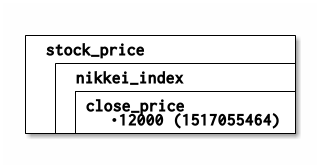
\includegraphics[width=8cm]{hoge.png}
\caption{Graphite example}
\end{figure}

\subsection{Datomic}
\label{sec:org3495517}
 Datomic は他のデータベースとはかけ離れた設計が行われた新しい世代の分散型データベースである。 Clojure の作者である Rich Hickey 氏らが作成し、有料でメンテナンスとアップデートが付属されたクラウドシステムを使うことができる。また一年に限っては無料でこの機能を利用することもできる。これとは別に存在する無料版に関しては分散できるピア数などの制限がかかる。\\
  Datomic には2つの目標「情報を時間によって紐付け蓄積する」 「データベースアプリケーションのモデルをリモートアクセスするものからそれぞれのプログラムの中にあるものとする」\footnote{http://endot.org/notes/2014-01-10-using-datomic-with-riak/} がある。この考え方によって得られた大きな2つの特徴に、\textcircled{\scriptsize 1} Append-Only \textcircled{\scriptsize 2}データベースに独立したクエリーエンジンがある。\\
 Append-Onlyとはその名の通り、追加のみという意味で、言い換えれば変更ができないということを意味する。これは情報を時間に紐付けることによって最新の情報を見ることができるため、情報を``書き換える''必要がなくなったためにできたことであり、トランザクション処理などのデータの管理を容易にすることができる。\\
 データベースに独立したクエリーエンジンとは、アプリケーション側でトランザクションやクエリ処理を実行するという意味を示しており、データベースに HTTP API などを用いてクエリを投げデータベース側がそのクエリを処理して結果を送信していたものをアプリケーション側に移す、ということになる。その意味で Datomic はアプリケーション側をピア \footnote{peer} と呼称する。\\
 ピアが扱うデータはデータベースではなくピア側のキャッシュに Read Only な形で LRU \footnote{Least Reacently Use}形式で保持される。データベースは書き込まれたデータを保存し、更新があればそれぞれのピアが持っている、データベースに対して常に開いているノードに告知し、アプリケーション側から要求されるデータ群をそのまま返すことになる。これによってピア側のメモリキャッシュを疑似データベースとして貪欲に使うことができ、データベースのボトルネックを解消することができるようになっている。更にピア側のキャッシュ上のデータベースは実質ゼロコストで用いることができるため、 LRU が最適であるような目的のアプリケーションにこのデータベースを適用した場合、データへのアクセスという点において他のデータベースに性能で劣ることはない。またクエリ処理を分散しているため、多くのクエリ処理をこなさなければならないピアが増えたとしても、キャッシュ上のデータを使っている限りはその処理によってデータベースに負荷がかかることもない。データベースの更新をピアに告知しなければならないという点でデータベースへの書き込みがネックになる可能性もあるが、論理的に分かれているデータごとにデータベースそのものを分割することで解決することができる。\\
 データベースのアクセス方法は Datalog と呼ばれる Clojure らしいシステムによって扱われるため、SQLに慣れている場合には苦労する可能性があるが、アプリケーションに柔軟に組み込むことができる。これはデータがキャッシュ上に Read-Only な形で存在しているという特性と、 Clojrue が関数型言語の側面を持っているという点を考えれば、データベース上のデータを手元にあるデータであるかのように利用することができるということを意味している。また保存しているデータは必ず Datom という最小単位に分割されており、これを元にして様々な形にデータを変形させることができる。\\
 このデータベースが扱うデータ例を以下に示す。\\

\begin{verse}
\{:nikkei-index/type ``close-price''\\
\hspace*{1em}:nikkei-index/value 12000\\
\hspace*{1em}:nikkei-index/timestamp 1517055464\}\\
\end{verse}
 データは nikkei-index/type に対する値として ``close-price'' が格納されている。nikkei-index に ``close-price'' が含まれているわけではない。\\

\begin{table}
\caption{Datomicの特徴}
\centering
\begin{tabular}{|c|l|}
\hline
目指すもの & \(\cdot\) 情報は時間によって紐付ける\\
 & \(\cdot\) データベースアプリケーションのモデルをそれぞれのプログラム内に移動する\\
\hline
大きな特徴 & \(\cdot\) Append-Only データベース\\
 & \(\cdot\) データベース側ではなくアプリケーション側にクエリ処理エンジンがある\\
\hline
\end{tabular}
\end{table}

\begin{figure}[htbp]
\centering
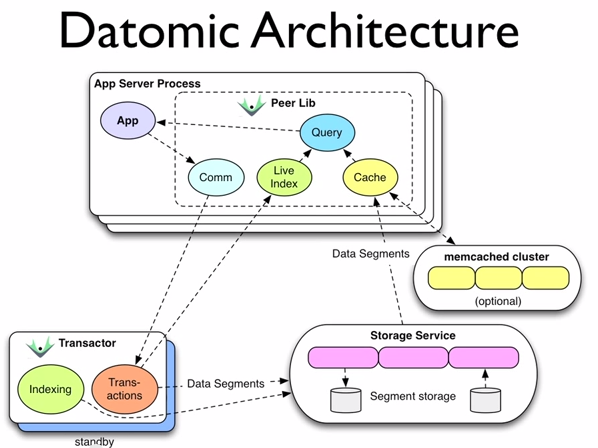
\includegraphics[width=15cm]{./datomic.png}
\caption{\href{http://endot.org/notes/2014-01-10-using-datomic-with-riak/datomic.png}{Talk Notes: Using Datomic With Riakより}}
\end{figure}

\newpage
\subsection{OpenTSDB}
\label{sec:org425ee64}
OpenTSDB の特徴の説明、セットアップや利用方法に関して説明を行う前に、その基盤である HBase とその周辺知識について簡単にまとめ、その後 OpenTSDB についての説明を行う。また OpenTSDB を用いる際に強力な可視化ツールとなる \href{https://grafana.com/}{Grafana} についてもデータベースの中身にデータが入っていることを示すために触れておく。\\

\subsubsection{HBase とその周辺知識}
\label{sec:org3279f1e}
HBase とは \(\href{http://hadoop.apache.org/}{Apache \textsuperscript{\texttrademark} Hadoop \textsuperscript{\textregistered}}\) (以降 ``Hadoop'' と呼称する) と呼ばれる、大規模データの分散処理フレームワークのためのデータベースである。そして Hadoop の分散サービスを形成するために \(\href{http://zookeeper.apache.org/}{Apache \ Zookeeper \textsuperscript{\texttrademark}}\) (以降 ``Zookeeper'' と呼称する)という管理ツールが使われる。\\
\subsubsection{HBase}
\label{sec:orgb778e7a}
HBase は NoSQL の一つである。NoSQL は大別して、\textcircled{\scriptsize 1}キーバリュー型\textcircled{\scriptsize 2}ワイドカラム型\textcircled{\scriptsize 3}ドキュメント型\textcircled{\scriptsize 4}グラフ型、があり HBase はワイドカラム型\footnote{簡単に説明するとデータを行ごとではなく列に対して管理しており特定の列を取り出して処理することに最適化されており、高いパフォーマンスやスケーラビリティを持っている。}に属している。\\

\begin{table}[htbp]
\caption{ワイドカラム型の例 (Name列を取り出すこと等を得意とする)}
\centering
\begin{tabular}{|c|c|c|c|c|}
\hline
ID & Name & Email & Birthday & Authorization\\
\hline
001 & Bob & bob @ foo.com & 1998/01/02 & true\\
002 & John & john @ bar.com & 1987/02/01 & false\\
\vdots & \vdots & \vdots & \vdots & \vdots\\
\hline
\end{tabular}
\end{table}

Hadoop の HDFS (Hadoop Distributed File System) の補完を担っており、複数台のマシンのディスクを一台のディスクであるかのように扱うことができる。全体のデータは Region という単位で分割されており、これをそれぞれのディスクに1つ以上割り振っていくことで分散を行う。\\
 続いて HBase の論理データモデルについて説明を行う。最上位概念は Namespace と呼ばれるもので、この中には Table と呼ばれるデータを表形式で保持している概念を1個以上含んでいる。Table は 一つ以上の RowKey 、一つ以上の ColumnFamily で構成されている。そして ColumnFamily には一つ以上の ColumnQualifier が存在している。行キーである ColumnQualifier と列キーである RowKey の交差点にはそれぞれ Cell と呼ばれる領域があり、ここにデータが格納されることになる。データは Timestamp とともに保存されており、 Cell にはそのデータが重ねて保存される。つまり Cell には Timestamp に紐付けられたデータが複数存在することになる。また、ワイドカラム型であるという特性上、Table は Rowkey でソートされた状態で保存されることになる。\\
 HBase の物理モデルの Table の構造はキーバリュー形式で保存されている。物理モデルの詳細はデータの分散などの説明も必要となるが、これ以上の内容は本演習で理解することができなかったため説明を省略する。\\

\begin{figure}[htbp]
\centering
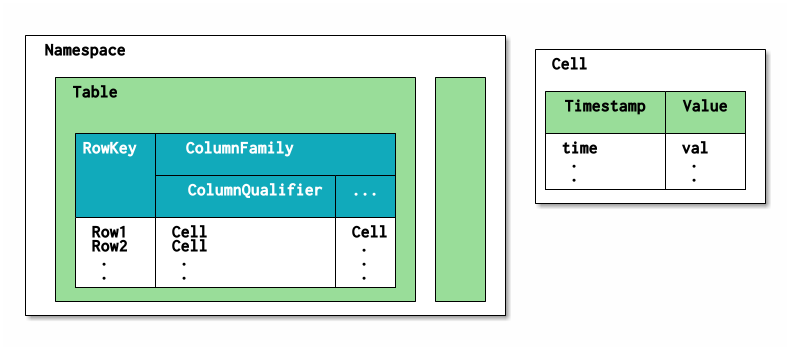
\includegraphics[width=.9\linewidth]{hoge2.png}
\caption{HBase の論理データモデル}
\end{figure}

\subsubsection{Hadoop}
\label{sec:orga922a28}
Hadoop は大規模データセットの分散処理フレームワークである。 Hadoop はモジュール化されているため、そのコンポーネントの殆どを別のソフトウェアに入れ替えることもできる柔軟な設計がされている。今演習では標準的な Hadoop の構成に付随してインストールされる、\textcircled{\scriptsize 1}Hadoop Common \textcircled{\scriptsize 2}Hadoop YARN\footnote{Yet Another Resource Negotiator} \textcircled{\scriptsize 3}Hadoop MapReduce \textcircled{\scriptsize 4}Hadoop Distributed File System (HDFS) をそのまま利用している。\\
 Common は他のモジュールに利用される基本的なライブラリ群である。 YARN は Hadoop のリソース管理やスケジューリングを行い、 MapReduce は分散処理のためのフレームワークである。 HDFS は分散ファイルシステムで、大容量ファイルを扱うことができる。HDFS は大量の小さなデータを高速に扱うことを不得手としているので、HBase がこの補完を行っている。\\
\subsubsection{Zookeeper}
\label{sec:orge09f29e}
Zookeeper は Hadoop などにおける、構成情報の管理、分散処理の提供、またグループサービスの提供なども行う、分散アプリケーション全体を管理するツールである。使用用途は多岐にわたり、例えば Hadoop などにおける構成管理、 \href{http://storm.apache.org/}{Apache Storm}\textsuperscript{\texttrademark} \footnote{リアルタイム高速分散処理フレームワーク} における処理の同期などに用いられる。ツリー状の階層化された名前空間を持ち、ノードと呼ばれる要素にサーバなどを割り当てている。高速処理や高い信頼性があるにもかかわらず、非常に簡単な API を持っていることが特徴である。ベンチマークとしては \href{http://zookeeper.apache.org/doc/current/zookeeperOver.html#fg_zkPerfRW}{Zookeeper\ 3.4\ Documentation} に記載されている。\\

\begin{figure}[htbp]
\centering
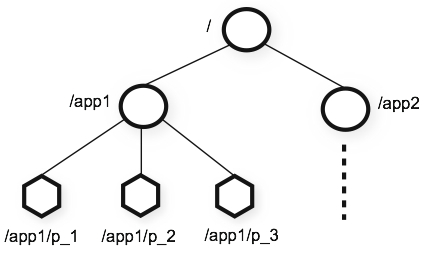
\includegraphics[width=8cm]{./zknamespace.jpg}
\caption{\href{http://zookeeper.apache.org/doc/current/zookeeperOver.html\#fg_zkPerfRW}{Zookeeperの階層構造}}
\end{figure}

\newpage

\subsubsection{OpenTSDB}
\label{sec:org6f2bfe2}
OpenTSDB とは HBase をホストとした \(\footnote {正確には Google の \href {https://cloud.google.com/bigtable/}{BigTable} もホストとなりうる}\) 時系列データベースで、その構成は\textcircled{\scriptsize 1} 時系列デーモン(以降 TSD と呼称する) \textcircled{\scriptsize 2} コマンドラインユーティリティ、の2つである。特徴としては TSD にマスター・スレーブといった上下関係がないこと、HBase などのホストに各アプリケーションが直接触れる必要がないこと、標準的に保存されているデータをブラウザから視覚的に確認することができることなどが挙げられる。\\
\begin{figure}[htbp]
\centering
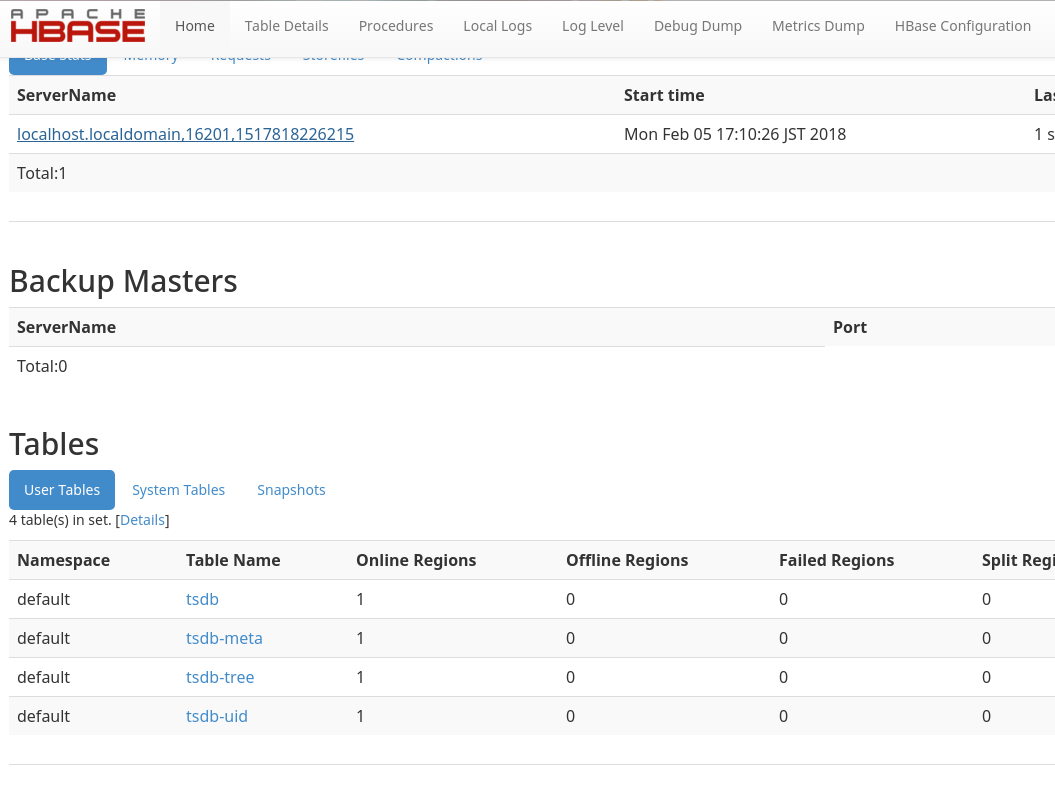
\includegraphics[width=15cm]{./hbase-view.PNG}
\caption{HBase 上の OpenTSDB (tsdb という名前のテーブルがあることが確認できる)}
\end{figure}

これによって得られる恩恵として、アプリケーションをチームで開発・維持する際に OpenTSDB を軸にしてデータベース側とアプリケーション側に分割することができるということが考えられる。例えばアプリケーション側はデータベース側の分散等の開発が終わる前に仮設置の HBase に対して OpenTSDB を適用し、アプリケーションをほぼ本環境と同じように動かすことができる。またデータベースの分散数を増やしたい場合は、データベース側にのみ視点を当てて変更を行うことができる。\\

\begin{figure}[htbp]
\centering
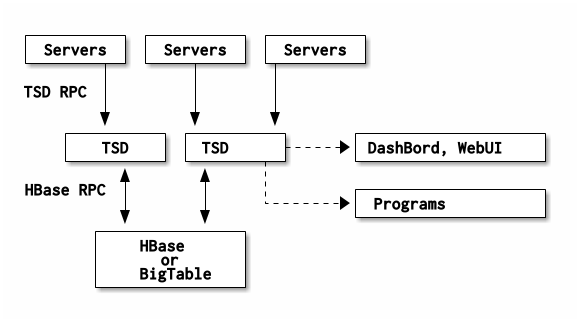
\includegraphics[width=10cm]{hoge3.png}
\caption{OpenTSDB の概略図}
\end{figure}

\newpage

OpenTSDB の論理モデルは Metric と呼ばれるその時系列データのタイトルとも言える概念が最も外側に位置しており、この中にテーブルに近い構造が一つ含まれていると考えることが出来る。このテーブルの行キーはソートされたタイムスタンプであり、時系列データベースの要である。テーブルの列キーはタグと呼ばれるキーバリュー形式の識別子が0以上割り当てられており、これによって欲しいデータの絞り込みを行うことができる。\\

\begin{figure}[htbp]
\centering
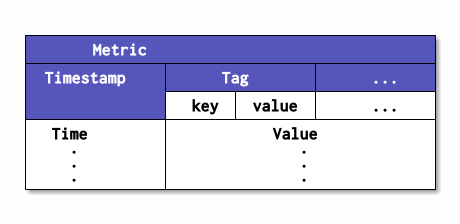
\includegraphics[width=12cm]{hoge4.png}
\caption{OpenTSDB の論理モデル}
\end{figure}

OpenTSDB はそのアクセスを HTTP API を用いて行うことができる。以降にその概要をまとめる。\\

\subsubsection{OpenTSDB の HTTP API}
\label{sec:orgf330a65}
OpenTSDB を利用するにあたって重要な要素に HTTP API の習得がある。このクエリによってアプリケーション開発者はデータの取得や送信を行うことになる。尚、HTTP API を使わずに Telnet を用いる手段もあるが、どちらも機能として同等であるためここでは HTTP API についての説明のみに留める。\\
 API は、データの取得に関してはクエリ文字列とボディ部の両方の手段をサポートしており、ボディ部を用いる場合はクエリ文字列を用いるよりも詳細な検索をかけることが出来る。対してデータの送信は PUT メソッドによるボディ部を用いた手段のみが利用できる。 それぞれの具体例を示すと以下のようになる。\\

\begin{table}[htbp]
\caption{OpenTSDBにおけるクエリ例\textcircled{\scriptsize 1}}
\centering
\begin{tabular}{|c|l|}
\hline
前提条件 & \(\cdot\) http: //localhost:4242 に対して OpenTSDB が開いている\\
クエリ内容 & 1年前から現在までの Metric nikkei-index における\\
 &  タグについてkeyが ``type'' 、valueが ``close-price''\\
 &  であるデータを要求する\\
\hline
クエリ文字列 & \(\cdot\) http: //localhost:4242/api/query $\backslash$\\
 &  ?start=1y-ago\&m=avg:nikkei-index\{type=close\_price\}\\
\hline
ボディコンテンツ & \(\cdot\) http: //localhost:4242/api/query\\
 & \(\cdot\) Content-Type JSON\\
 & \(\cdot\) Body\\
 & \{ "start" : 1y-ago,\\
 &  "queries" :\\
 &   [\{"aggregator" : "sum",\\
 &      "metric" : "nikkei-index",\\
 &       "tags" :\\
 &        \{"type" : "close-price"\}\\
 &  \}]\\
 & \}\\
\hline
\end{tabular}
\end{table}

\begin{table}[htbp]
\caption{OpenTSDBにおけるクエリ例\textcircled{\scriptsize 2}}
\centering
\begin{tabular}{|c|l|}
\hline
前提条件 & \(\cdot\) http: //localhost:4242 に対して OpenTSDB が開いている\\
クエリ内容 & \(\cdot\) Metric ``nikkei-index'' の、\\
 &  タグが、key は``type''、value は``close-price'' である\\
 &  UnixTime が 1717055464 である時間に、\\
 &  12000 という値を保存する\\
\hline
 & \(\cdot\) http: //localhost:4242/api/put\\
 & \(\cdot\) Content-Type JSON\\
 & \(\cdot\) Body\\
 & \{ "metric" : "nikkei-index",\\
 &  "timestamp" : 1717055464,\\
 &  "value" : 12000,\\
 &  "tags" :\\
 &    \{"type" : "close-price"\}\\
 & \}\\
\hline
\end{tabular}
\end{table}

\newpage
\subsubsection{Grafana}
\label{sec:orgd3874ad}
 Grafana は InfluxDB や Graphite 、 OpenTSDB などのデータベースに対してデータを視覚化させるためのツールで、 Web ブラウザから Grafana が開けることになるポート\footnote{標準では3000番}にアクセスすることで、ユーザーフレンドリーなクエリ処理機構を用いてデータベースと通信を行い、得られた結果をグラフや表にすることができる。以下にその例を示す。\\
\begin{figure}[htbp]
\centering
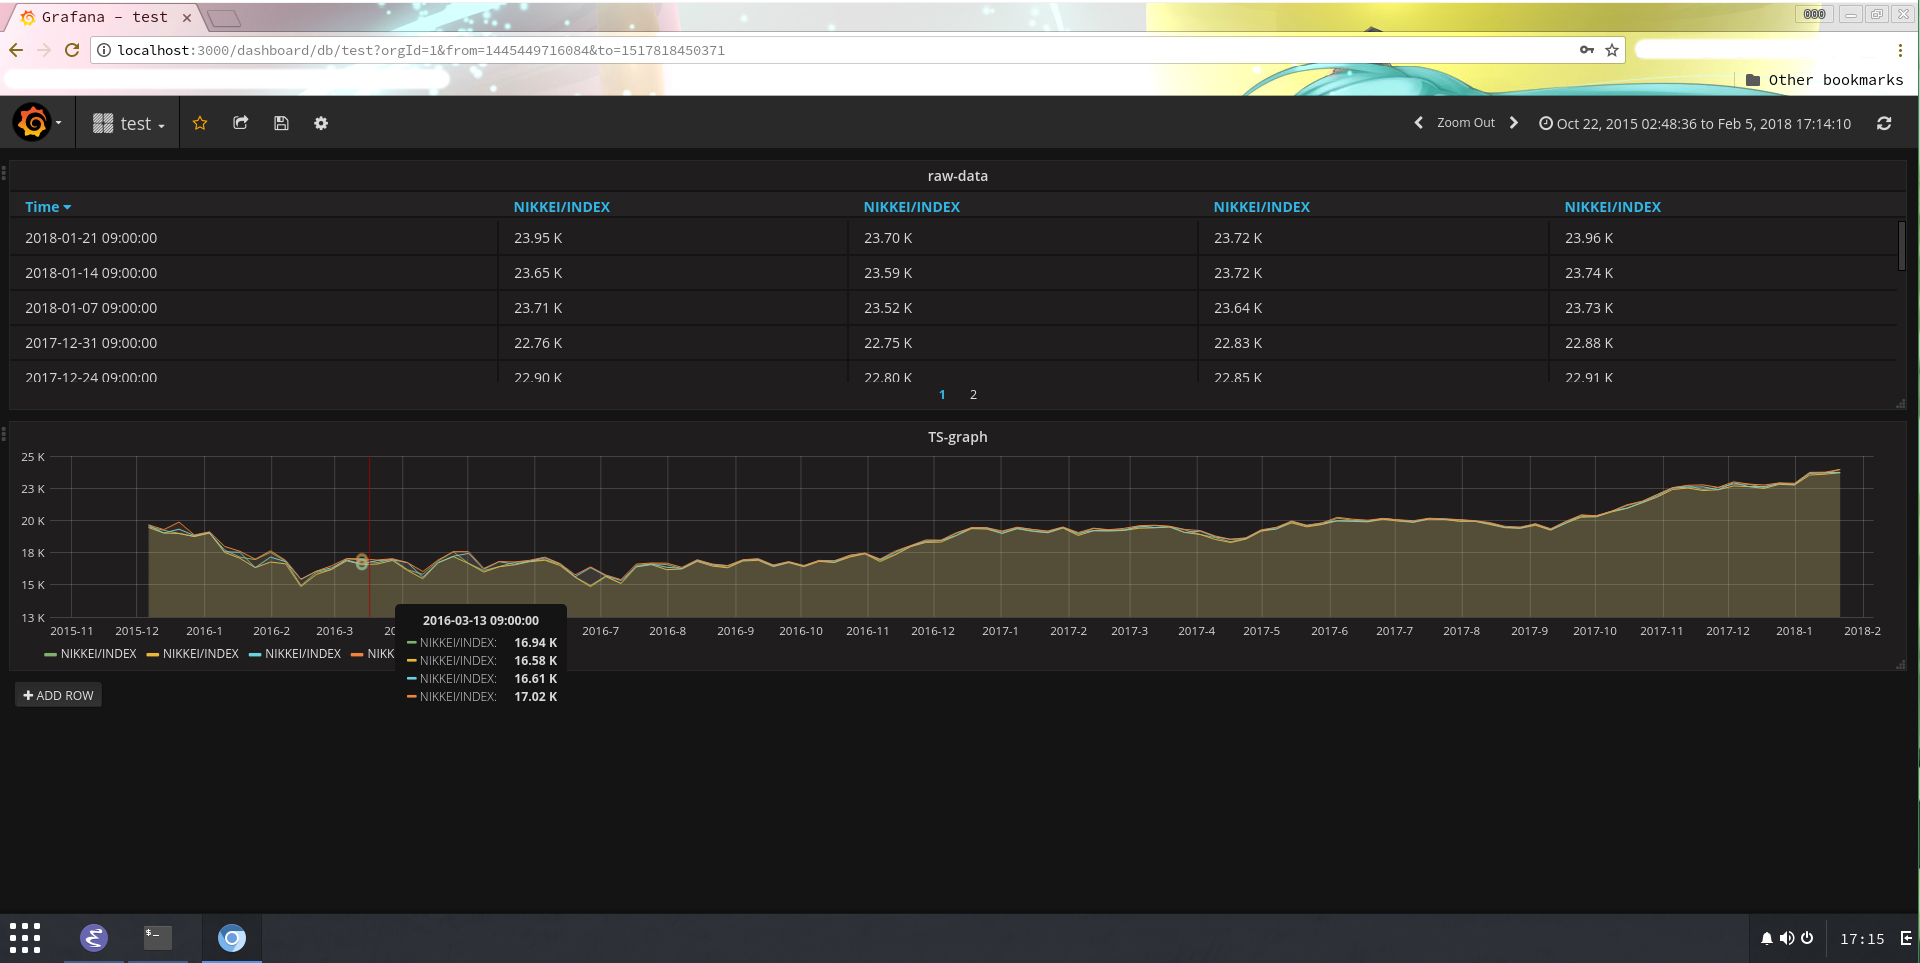
\includegraphics[width=15cm]{./grafana.PNG}
\caption{Grafana を用いた視覚化の例}
\end{figure}
\newpage
\section{Clojure を用いた JVM における高速計算技法}
\label{sec:org9a4b90f}
本演習の開始時、自分のこれまでのプログラム言語学習経歴 \footnote{昨年の情報特別演習においてはPythonを中心に利用し、授業外で Common Lisp をある程度習得した} から、 Lisp の影響を受けた言語を選択することが最も演習に適していると考えており、更に HBase を活用することが決定していたため、 \href{https://www.java.com}{Java} に近く Lisp に近い言語として JVM \footnote{Java virtual machine}上で動作する \href{https://clojure.org}{Clojure} を採用した。また演習を勧めていく上でフロントエンドの開発も行う必要が出てきたため、同様のシンタックスを用いる \href{https://clojurescript.org}{ClojureScript} も採用し、この両方の言語を中心に学習した。\\
 この章ではその内の Clojure における高速計算手法についての学習成果を完結にまとめる。\\

\subsection{Clojure 自身の高速化手法}
\label{sec:org084c936}
Clojure に GPU ライブラリ等を適用する以前に純粋な Clojure で最適化されたコードを書くことが高速計算を行う際に重要であることは言うまでもない。本演習では Clojure 自身の学習も兼ね Clojure for the Brave and True \cite{Brave} 、Clojure High Performance Programming \cite{high-performance} を教材に Clojure の最適化手法を学習した。具体的な学習内容としてはプログラム設計の見直しや基本的なシンタックスの見直し、効率の良いスレッド化・並列処理、プログラム全体のパフォーマンス測定法(プロファイリング法)などである。成果としてどこまでの性能向上が認められたかを具体的に比較することは難しいが、性格の良いプログラムを書くことが出来るようになったのではないかと考えている。\\

\subsection{ClojureCL}
\label{sec:org40525b4}
\href{http://clojurecl.uncomplicate.org/}{ClojureCL} とは Clojure で OpenCL を用いるためのライブラリで C言語で書かれる OpenCL のコードよりも簡潔なシンタックスで書くことが主張されている。このライブラリはJVM上でOpenCLを動作させるため、 JNI\footnote{Java Native Interface} を基盤としたライブラリである jocl を用いており、非常に低レベルな部分で OpenCL とリンクしているため、OpenCL そのものの知識が必要となるものの、その速度を十分に体感することが出来る。本演習ではドキュメントに記載されたソースコードを移し、自分の環境においてそれを体験するまでを行った。2018年2月1日においてはより深い理解を行うために、OpenCL in Action \cite{OpenCL} を学習している。\\

\subsection{Neanderthal}
\label{sec:org7849ef4}
\href{http://neanderthal.uncomplicate.org/}{Neanderthal} は、Intel \textsuperscript{\textregistered} MKL を用いた高速行列演算・線形代数のためのライブラリである。その速度はGPUを利用するモードの場合には大規模サイズの行列演算に関しては、 Clojure / Java ライブラリに対しても大凡3000倍の高速化を達成し、CPUを利用する場合においても純粋な Java よりも 100 倍の高速化を達成している。このライブラリは後述する Clojure.core.matrix 系ライブラリに対してやや扱いが難しいが、その分大幅な高速化が望むことが出来る。またこのライブラリの依存関係は intel MKL のライブラリ を含むことに意味があるため、 intel MKL のライブラリ \(\footnote{Arch Linuxにおいては /opt/intel/lib,/opt/intel/mkl/lib }\) をアプリケーション内に含んでしまえば標準的な環境で動作させることが出来る。\\

\begin{figure}[htbp]
\centering
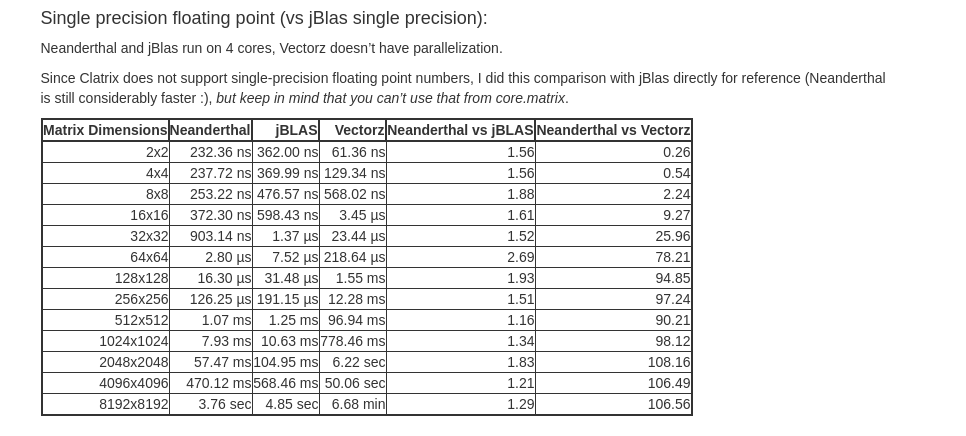
\includegraphics[width=15cm]{./neanderthal.png}
\caption{ベンチマーク \href{http://neanderthal.uncomplicate.org/articles/benchmarks.html}{Neanderthal Benchmarks} より}
\end{figure}

\newpage
残念ながら本演習では成果物を稼働させるサーバをどのように扱うかについて協議が不足しており、更に必要とされるライブラリがその環境で利用可能であるか不明であったため、実装に組み込ませることができなかった。しかし積極的にこちらを用いて開発を行いたいと考えている。ここで実行例の一部を紹介する。\\

\captionof{listing}{test-Neanderthal.clj}
\begin{minted}[frame=lines,linenos=true,obeytabs,tabsize=4]{clojure}
(ns test-neanderthal.core
  (:require
   [uncomplicate.neanderthal.core :refer :all]
   [uncomplicate.neanderthal.native :refer :all]
   [uncomplicate.neanderthal.linalg :refer :all]))

;; ------------------------------------------------------------
;; sample1
(def a (dge 2 3 [1 2 3 4 5 6]))
;; #RealGEMatrix[double, mxn:2x3, layout:column, offset:0]
;;         ↓       ↓       ↓       ┓
;; →       1.00    3.00    5.00
;; →       2.00    4.00    6.00
;; ┗                               ┛

(def b (dge 3 2 [1 3 5 7 9 11]))
;; #RealGEMatrix[double, mxn:3x2, layout:column, offset:0]
;;         ↓       ↓       ┓
;; →       1.00    7.00
;; →       3.00    9.00
;; →       5.00   11.00
;; ┗                       ┛

(mm a b)
;; #RealGEMatrix[double, mxn:2x2, layout:column, offset:0]
;;         ↓       ↓       ┓
;; →      35.00   89.00
;; →      44.00  116.00
;; ┗                       ┛

;; ------------------------------------------------------------
;; sample2
(def A (dge 3 2 [1 0 1 1 1 2]))

(def or (qrfp A))
;; #RealGEMatrix[double, mxn:3x2, layout:column, offset:0]
;;         ↓       ↓       ┓
;; →       1.41    2.12
;; →      -0.00    1.22
;; →      -2.41    3.15
;; ┗                       ┛

(def r (dge 2 2 (:or or)))
;; #RealGEMatrix[double, mxn:2x2, layout:column, offset:0]
;;         ↓       ↓       ┓
;; →       1.41    2.12
;; →      -0.00    1.22
;; ┗                       ┛

(def q (org or))
;; #RealGEMatrix[double, mxn:3x2, layout:column, offset:0]
;;         ↓       ↓       ┓
;; →       0.71   -0.41
;; →       0.00    0.82
;; →       0.71    0.41
;; ┗                       ┛

(def b (dge 3 1 [1 0 -2]))

(def x (mm (tri (trf r)) (trans q) b))
;; #RealGEMatrix[double, mxn:2x1, layout:column, offset:0]
;;         ↓       ┓
;; →       1.00
;; →      -1.00
;; ┗               ┛

;; ------------------------------------------------------------
;; sample2 ~another solution~
(def A (dge 3 2 [1 0 1 1 1 2]))

(def b (dge 3 1 [1 0 -2]))

(def x_ (dge 2 1 (ls A b)))
;; #RealGEMatrix[double, mxn:2x1, layout:column, offset:0]
;;         ↓       ┓
;; →       1.00
;; →      -1.00
;; ┗               ┛
\end{minted}

\newpage
 5行目までの内容は依存関係の解決である。 Sample1 において単純な行列の掛け算を行っており、 Sample2 は QR 分解を用いて \(Ax = b\) の解を求めている。そして Sample2 \(\sim\) another solution \(\sim\) はこれを存在しているライブラリ関数を用いて解いたものである。両者の速度差はこのサイズの行列演算であればほぼないが、大規模サイズの行列であった場合は後者のほうが圧倒的に速い。後者も前者もほぼ直接 Fortran のライブラリである \href{http://www.netlib.org/lapack/}{LAPACK} \(\footnote{\href{http://www.netlib.org/lapack/}{Linear\ Algebra\ PACKage}}\) を触っているため、計算途中で結果を取り出している前者のほうが効率が悪いためである。\\
 このコードからわかるように、このライブラリが返す値は必ずしも求めている/求まった解答の形を示していない。この理由は Intel MKL 内のソースコードが与えられたデータのメモリに解答を書き込む性質があるためである。この破壊的代入を行う性質は高速化に大きな貢献をしているとともに、高い副作用と難解さを招いている原因であると考えられるが、このライブラリを利用するためには Intel MKL のドキュメントを精読することや、内部の Fortran による実装を眺める他にない。\\

\subsection{Clojure.core.matrix}
\label{sec:orga0d64c8}
 先に紹介した2つに対してこちらは非常におとなしいライブラリであり、 Clojure の標準的な算術関数のラップや行列演算に関するライブラリの基盤を開発している。ライブラリの基盤というのは、 Java などのオブジェクト指向言語におけるインターフェースのようなもので、実装するべき関数を先に示しておくことで、それを様々な手法によって実装・更新されていくことで長期的にそのライブラリ群を使うことが出来るという利点がある。本演習では、高速さが持ち味である \href{https://github.com/mikera/vectorz-clj}{vectorz-clj} や、 \href{http://jblas.org/}{jblas} を用いて実装されており更に関数が充実している \href{https://github.com/tel/clatrix}{clatrix} の2つを検討し、その両方を利用した。\\

\subsubsection{vectorz-clj}
\label{sec:org1eada2e}
 Vectorz-clj は純粋に JVM で動作する高速な行列計算ライブラリを掲げており、導入にかかるコストの低さが魅力的である。問題としては行列の結合・切り出しに関する関数のいくつかの挙動が不自然であることで、その点を除いては後述する clatrix よりも概ね高速に動作する。\\
\subsubsection{clatrix}
\label{sec:orgc003192}
 clatrix は jblas をラップしたライブラリであり、行列計算において必要とされる関数をほぼすべて網羅しており、先述のライブラリで不足した部分を補完するために利用した。このライブラリを利用するためには jblas がインストールされていることが必要であるため、標準的な環境にこれを用いたアプリケーションを実行したとしても正常に動作しない。不足する関数を自力で補完することでこのライブラリを使用しないという選択肢もあるため、よりアルゴリズムの能力を磨いて自力で必要な関数を補完したいと考えている。\\

\subsection{ACM3 (Apache Common Math 3)}
\label{sec:org52d9eac}
 計算速度そのものの向上という意味ではこのカテゴリからはやや離れるが、良質なアルゴリズムを用いている様々な数学に関するライブラリとして ACM3 がある。本演習ではそのうちの、アメーバ法に関する関数を ARMA モデルにおけるパラメータ推定のために利用した。\\
\section{ARIMA モデルによる時系列分析}
\label{sec:org73bc3ce}
 (S)ARIMA モデルは時系列分析手法の一つであり、本演習の要とも言える機械学習手法である。本演習ではこのモデルとその周辺手法を実装した。\\
 ARIMA モデルは 正確には ``Autoregressive integrated moving average model'' と呼ばれ、概要は \textcircled{\scriptsize 1} I \textcircled{\scriptsize 2} AR \textcircled{\scriptsize 3} の3要素によって構成されており、この適用できるデータは「非定常過程が見られる」時系列データ \footnote{「定常過程を持っている」時系列データは ARMA (Autoregressive moving average) モデルでの推定となる} である。定常過程と非定常過程の違いについては後述する \ref{sec:orgb7042aa} 単位根検定 で説明を行うが、時系列データには非定常過程を持っている場合が少なからずあり、更に ARIMA モデルを ARMA モデルに変換することは非常に容易であるため ARIMA モデルを実装することによって実質的に定常過程、非定常過程両方の性質を持った時系列データを分析することが出来る。尚 ARIMA モデルの分析対象はある時系列データ内の時点間の関係である、自己相関 \footnote{系列相関ともいう} にある。\\
 また ARIMA モデルの発展として季節階差を削除することを目的とした SARIMA モデルもあるが、こちらは \ref{sec:orgf282bf4} SARIMA モデルについて にある理由により開発を中断した。\\
 以降にこのモデルの実装において必要になる知識を紹介する。尚ここで使用する式の書式に関しては \ref{sec:orgf55781c} 付録に記載する。\\

\subsection{BackShift記法}
\label{sec:org8b1e7a2}
 BackShift記法とは、記号 ``B'' という演算子を用いた時系列データを表現するための手法であり、以下のような使われ方をする。\cite{otext}
\begin{align}
(1-B)Y_t &= 1  Y_t - B  Y_t = Y_t - Y_{t-1} \\
(1-B)^2 Y_t &= (1-B)  (1-B) Y_t \\
(1-B^k) Y_t &= Y_t - B^k  Y_t \nonumber \\
&= Y_t - Y_{t-k}
\end{align}
 但し \(Y_t\) は時系列データを表しており、また今後の説明のため、tが大きいほど最近のデータであるものとする。\\
 式(1) は一次階差を表しており、後述する AR モデルでは AR(1) の場合に用いられる。式(2) は二次階差を表しており、同様に AR(2) の場合に用いられる。式(3) はある区間を開けて階差を取っており、これは季節階差を取る際等に用いられる。季節階差という考え方から一旦離れてわかりやすい例を挙げるとすれば、時系列データが月単位のデータであった場合、昨年と今年の差分を取る場合には、 \((1-B^{12})Y_t\) という形をとることになる。\\
 この記法を用いることでn次階差や季節階差を表しやすくなり、また関数型言語などにおいてはその実装の手がかりを得ることが出来る \footnote{$(1-B^n)$という意味を持つ関数を定義することで理論上ARIMAモデルに必要な階差に関する関数は満足することが出来る}。\\

\subsection{単位根検定}
\label{sec:orgb7042aa}
 実世界に存在する多くの時系列データは非定常過程を持っていることが示唆されている。この示唆について Jackknifing multiple-window spectra \cite{389899} から有名な一説を引用すると以下のようになる。\\
\begin{verse}
Experience with real-world data, however, soon convinces one that both stationarity and Gaussianity are fairy tales invented for the amusement of undergraduates.\\
\vspace*{1em}
- Thomson, 1994\\
\end{verse}

 ARIMA モデルでは「非定常な」時系列データを 階差 を取ることによって「定常な」時系列データに変換し ARMA モデルに適用する。ARIMA モデルにおける I 部分には d 次の階差を取るという意味が含まれている。一般にこの階差は一次であるらしいが、実装側では以降に紹介する ADF検定 をおこなうことで定常性を判定した。またこの他にも、KPSS 検定や Ljung-Box 検定などがあるが、単位根検定という観点から KPSS 検定のみを追加で紹介することとする。\\

 以降における \(y_t\) について定義する。 \(Y_t\) を議論の時系列データとして、\\
\begin{align}
y_t = Y_t - E(Y_t) = Y_t - \mu - \mu_1 t
\end{align}
 正確ではないが、ここにおける \(\mu\) は \(t = 0\) における時系列データの値、 \(\mu_t\) は 時系列データの傾きと考えることが出来る。\\

\subsubsection{定常性の性質}
\label{sec:org434eb10}
 ここまで``定常性''という言葉を多用してきたが、この定常性について簡単に触れておく。定常性とは同時分布が時間を通じて変わらないこと \footnote{この同時分布が同一であることを持つ時系列過程を特に``強定常である''という} を意味しており、以下のような性質を持っている。\\

\begin{itemize}
\item \(E(Y_t) = \mu\) \\
 母平均 (population mean) は時点 t に依存しない。\\
\item \(Var(Y_t) = \gamma_0\) \\
 分散 (variance) は 時点 t に依存しない\\
\item \(Cov(Y_t, Y_{t-j}) = \gamma_j\) \\
 共分散 (covariance) は 時点 t に依存しない \footnote{$\sigma_{Y_t Y_{t-j}}$と表すこともある}
\end{itemize}

 更に \(E(Y_t) = \mu \land Cov(Y_t, Y_{t-j}) = \gamma_j\) のみである場合を特に``弱定常である''という。\\

 逆に非定常過程の時系列データに目を向けたとき、経済学上重要な要素に以下のようなものがある。\\
\begin{itemize}
\item 確定的トレンド (deterministic trend)\\
  \(Y_t = \beta t + \epsilon_t \ where \ \epsilon_t \sim iid(0, \sigma^2)\) と表され、\(E_{DT}(Y_t) = \beta_t\) 、 \(Var_{DT}(Y_t) = \sigma^2\) である。こちらは直ちにトレンド定常 (trend stationarity) という形に変形することが出来る。\\
\item 確率的トレンド (stochastic trend) 又は単位根過程\\
  \((1-B)Y_t = \beta + \epsilon_t \ wherer \ \epsilon_t \sim iid(0,\sigma^2)\) と表され、 \(E_{ST}(Y_t) = \beta_t\) 、 \(Var_{ST}(Y_t) = t \sigma^2\) である。\\
 確定的トレンドに比べこちらは時間が経過する程に大きな影響を及ぼすことになる。こちらは後述する単位根検定として利用できる ADF 検定や KPSS 検定を行うことで発見することが出来る。\\
\item 構造変化\\
 その時系列が予期しない変化(経済データであるならば、例えば突発的な戦争や飢餓)を受けた際に起こる。本来はこれに対する検定も用意するべきであったが、どのような条件をフラグとして検定が行われるべきであるかが理解できなかったため実装することができなかった。\\
\end{itemize}

\begin{figure}[htbp]
\centering
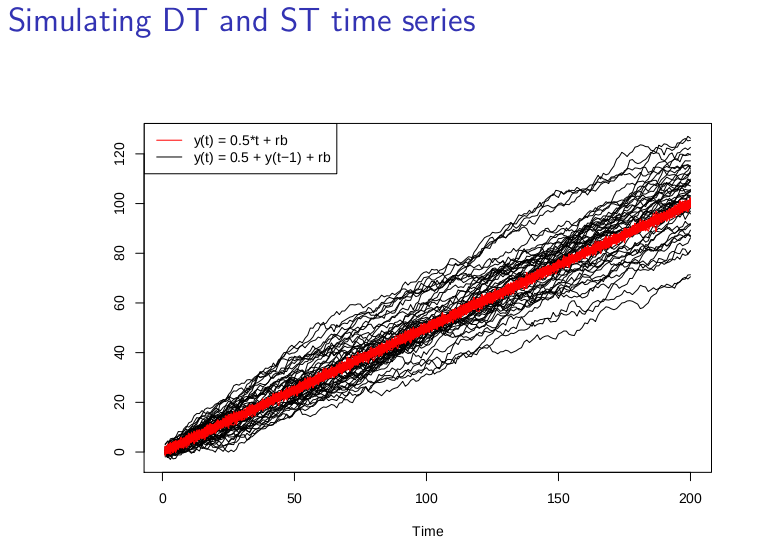
\includegraphics[width=16cm]{./hedibert.png}
\caption{difference between Deterministic and Stochastic trend \cite{hedibert}}
\end{figure}

\newpage
\subsubsection{ADF 検定}
\label{sec:org509e8ed}
 ADF 検定 (Augumented Dickey-Fuller test) は DF 検定 (Dickey-Fuller test) の拡張である。\\
 DF 検定とは \(Y_t\) について自己回帰モデル AR(1) を作成し以下の条件を用いて仮説検定を行う手法である。\\
 AR(1)モデル \(Y_t = \theta Y_{t-1} + \epsilon_t \  where \ \epsilon_t \sim iid(0, \sigma^2)\) とする。(AR モデルそのものについては \ref{sec:org0622dbe} AR モデル で解説を行う)\\
 単位根を持っていることを帰無仮説とし、定常であることを対立仮説であるとする。\\
 つまり、帰無仮説 \(H_0\) と対立仮説 \(H_A\) は以下のように定義できる\\
\begin{align}
H_0\ :\ \theta = 1 \\
H_A\ :\ \theta < 1
\end{align}
 ここからモデルを変形し、以下の式を立てる。\\
\begin{align}
\Delta Y_t = (\theta - 1) y_{t-1} + \epsilon_t   
\end{align}
 上式において、\(\pi = (\theta - 1)\) と置換した場合、帰無仮説と対立仮説は以下のように更新される。\\
\begin{align}
H_0\ :\ \pi = 0 \\
H_A\ :\ \pi < 0
\end{align}
 この検定値は簡単な t 検定によって求めることが出来、以下の式によって得られる。\\
    \begin{align}
\widetilde{\tau} &= (\hat{\theta} - 1) / {se(\hat{\theta})} \nonumber \\ 
                 &= \hat{\pi} / se(\hat{\pi})
    \end{align}
 これを自ら指定した有意水準(5\% 又は 1\% であることが多い) において検定する。この検定手法では対立仮説が成り立つならば定常性を認めることが可能である。混乱を招かないために強調するが、この検定における帰無仮説は、``単位根を持っている''ことである。これが棄却されれば``定常である''ことを認めることができる。\\
 また上の場合において、元データの一次階差と取っていることが明らかであるが、この検定で定常であると認められた場合、このデータは 1次の単位根 があるという。同様に d次の単位根がある とは、d - 1 次までの単位根検定においてすべて 非定常である と判断され、 d 次において初めて 定常である と判断されたことを示している。\\
 DF 検定が AR(1) モデルに対する検定であることにたいして、ADF 検定は AR(n) モデルにまで対象を拡大したものであり、一般式は難解であるため省くが、例えば AR(3) モデルは以下のように示すことが出来る。\\
   \begin{align}
   Y_t &= \theta_1 Y_{t-1} + \theta_2 Y_{t-2} + \theta_3  Y_{t-3} + \epsilon_t \ where \ \epsilon_t \sim iid(0,\sigma^2) \\
   Y_t - Y_{t-1} &= (\theta_1 - 1) Y_{t-1} + \theta_2  Y_{t-2} + \theta_3  Y_{t-3} + \epsilon_t \\
   \Delta Y_t &= (\theta_1 + \theta_2 + \theta_3 - 1)  Y_{t-1} \nonumber \\
&+ (\theta_2 + \theta_3) (Y_{t-2} - Y_{t-1}) + \theta_3 (Y_{t-3} - Y_{t-2}) + \epsilon_t \nonumber \\
&= (\theta_1 + \theta_2 + \theta_3 - 1) Y_{t-1} + (\theta_2 + \theta_3) * \Delta Y_{t-1} + \theta_3 \Delta Y_{t-2} + \epsilon_t
   \end{align}
 これより \(\pi = (\theta_1 + \theta_2 + \theta_3 - 1)\) とおいて DF 検定と同様に t 検定を行う。\\
 尚この検定にはいくつかの追加要素として、定常過程にある時系列データの平均値を考えるパターンや、時系列データに傾きがある場合を考慮したパターンがある。これらは人為的にデータを確認することで決定するが、 R 言語や Python などの ADF 検定ではすべてのパターンを一度に実行している場合がある。これは ADF 検定そのものは計算コストが低いため、すべてのパターンを網羅しても問題がないためである。\\
\subsubsection{KPSS 検定}
\label{sec:orgc451067}
 KPSS 検定 (Kwiatkowski-Phillips-Schmidt-Shin test) とは先述の ADF 検定に対して帰無仮説と対立仮説を反転させたものとイメージすることが出来る。この検定においては以下の式を中心に展開する。\\
\begin{align}
Y_t &= \xi_t + \epsilon_t \nonumber \\
 &where \ \xi_t = \xi_{t-1} + \upsilon_t \nonumber \\
 &\ \ \ \ \ \ \upsilon_t \sim iid(0, \sigma_{\upsilon}^2) \nonumber \\
 &\ \ \ \ \ \ \epsilon_t \sim iid(0, \sigma^2)
\end{align}
 この式における \(\xi_t\) はランダムウォークを示している。尚ランダムウォークとは次に現れる値が確率的にランダムであることを示す。また、\(\epsilon_t\) はその性質から定常過程を示している。\\
 仮に \(\sigma_{\upsilon}^2 = 0\) であるとしたとき、\(\xi_t = \xi_0\) であることから上式に影響を加える要素は \(\epsilon_t\) のみとなり、つまり \(Y_t\) は定常であるとみなすことが出来る。これを用いて上式を変形すると以下のようになる。\\
\begin{align}
Y_t = \hat{\mu} + \hat{\epsilon_t}
\end{align}
 ここで仮説検定を行う。帰無仮説は 定常過程を示している式(15)であり、つまりは式(14) における \(\sigma_{\upsilon}^2 = 0\) である。対立仮説はこの逆であり、非定常であること、つまり \(\sigma_{\upsilon}^2 > 0\) である。\\
\begin{align}
H_0 \ :\ \sigma_{\upsilon}^2 = 0 \\
H_0 \ :\ \sigma_{\upsilon}^2 > 0
\end{align}
 検定は以下の式を用いて行う。\\
\begin{align}
KPSS &= 1/T^2 (\Sigma^{T}_{t = 1}S_t^2)/ \hat{\sigma^2_\infty} \nonumber \\ 
&where\  S_t = \Sigma_{s=1}^t \hat{e_s} 
\end{align}

 また上式における \(\hat{\sigma^2_\infty}\) とは \(\epsilon_t\) の長期変動に関する HAC 推定量 \footnote{特に Newey-West 推定量を用いられることが多い} である。\\
 以下に \(\sigma^2_\infty\) の例を示す。\cite{STAN:STAN272}
\begin{align}
\sigma^2_\infty = \lim_{T \rightarrow \infty} (1/T E((\Sigma_{t=1}^T \epsilon_t)^2))
\end{align}
 ADF 検定あったようにこちらにもいくつかのパターンがあり、トレンド定常の場合などの場合に合わせた形に 式(14) が存在し、それに伴って仮説検定の内容に多少の変化がある。\\
  実装においては HAC 推定量を理解・実装することができなかったため、KPSS検定も実装することができなかった。\\
\subsection{AR モデル}
\label{sec:org0622dbe}
 AR(p) モデル (自己回帰モデル) は以下の式で表すことが出来るモデルである。重回帰モデルが説明変数の線型結合を用いて関心のある変数を予測していること対して、自己回帰モデルは説明変数を過去の観測値に置き換えたものであると言える。\\
\begin{align}
Y_t &= c + \phi_1  Y_{t-1} +\phi Y_{t-2} + \cdots + \phi_p  Y_{t-p} + \epsilon_t \nonumber \\
&= c + \Sigma_{i=1}^{p} (\phi_i  Y_{t-i}) +\epsilon_t  \nonumber \\
&where \  c \ is\  constant \ \nonumber \\ 
&\ \ \ \ \ \ \ \ \ \ \epsilon \sim iid(0, \sigma^2)
\end{align}
 式からわかるように \(c\) は定数項である。\\
\subsection{MA モデル}
\label{sec:orgfd8eb6e}
 MA(q) モデル (移動平均モデル) は以下の式で表すことが出来るモデルである。同様に重回帰モデルの説明変数を過去のノイズの重みに置き換えたものであると言える。これとよく似たものに移動平均という手法があるが、移動平均は過去の値のサイクルを推定するために用いられ、MA(q) モデルは将来の値を予測するために用いられる。\footnote{移動平均とMAモデルは正確には別のものであり、混同されるべきではない。MAモデル自体は有限インパルス応答に近い発想である。\cite{2012カルマンフィルタの基礎}}

\begin{align}
Y_t &= c + \epsilon_t + \theta_1 \epsilon_{t-1} + \theta_2 \epsilon_{t-2} + \cdots + \theta_1 \epsilon_{t-q}   \nonumber \\
&= c + \epsilon_t + \Sigma_{i=1}^{q} (\theta_i \epsilon_{t-i})  \nonumber \\
\end{align}
\subsection{ACF と PACF}
\label{sec:orga0d47cc}
 ARMA モデルにおいて\footnote{ACF, PACFは定常過程であるデータに適用される}、AR(p), MA(q) の p, q の値を決定する際の指標となるものに、ACF、PACFがある。この2つはグラフによって視覚化され、この2つのグラフから p, q の値は手動で決定される。\footnote{R言語における auto.arima 関数などはこのような手間なしでモデルを決定することが出来るが、これは p, q などの値を元データにかかわらず適当に複数定めモデルを作成し、AICなどを用いて最も良いモデルを選択しているからである。} \cite{stat510}
\subsubsection{ACF}
\label{sec:orgf2068da}
 ACF (autocorrelation function) は自己相関係数とも呼ばれ、元データとある時点分だけずらしたデータとの相関係数を計算する。つまり以下の式を計算することになる。尚 \(t-s\) はそのずらした量(ラグと呼ぶ)である。またこの場合に求まる値を、\(t-s\) 次のACFと呼ぶことがある。\\
\begin{align}
\rho(s,t) &= (E((Y_t - \mu_t)(Y_s-\mu_s)))/(\sigma_{Y_t}\sigma_{Y_s}) \nonumber \\
&= (E((Y_t - \mu_t)(Y_s-\mu_s)))/\sigma^2 \nonumber \\
&= Cov(Y_t, Y_s)/\sigma^2
\end{align}
 上式では \(\sigma_t\sigma_s = \sigma^2\) が成り立っている。これは定常過程を持つ時系列データの分散が時点に依存しないためである。\\
 尚 ACF と PACF には閾値があり、この閾値を超えた値を元に p, q を考えていく。以下にその境界値を求める式を示す。 但し n はデータサイズである。\\
\begin{align}
threshold = \pm 2/\sqrt{n}
\end{align}
\subsubsection{PACF}
\label{sec:org932d182}
 PACF (partical autocorrelation function) は偏自己相関とも呼ばれ、ある時点とそこからある時点分だけ離れた時点の二点間の、その間の存在の影響も考慮した場合における相関関係である。一般式は複雑であるため、2次、3次の 偏自己相関 の式を示す。尚、1次の PACF は 1次の ACF に等しい。計算の都合上、k次の 偏自己相関 を \(\phi(k, k)\) と表す。\\
\begin{align}
\phi(2, 2) &= Cov(Y_t,Y_{t-2}|Y_{t-1}) / (\sigma_{Y_t|Y_{t-1}} \sigma_{Y_{t-2}|Y_{t-1}}) \\
\phi(3, 3) &= Cov(Y_t,Y_{t-3}|Y_{t-1},Y_{t-2})/(\sigma_{Y_t|Y_{t-1},Y_{t-2}}\sigma_{Y_{t-3}|Y_{t-1},Y_{y-2}})
\end{align}
 このように式がラグごとに異なるため、実装上計算には以下の行列式を用いた Durbin-Levinson recursion が用いられることが多い。尚 以下の式における \(\rho(s)\) とは 自己相関 \(\rho(s, t)\) を示している。\\
\begin{equation}
\left(\begin{array}{ccccc}
\rho(0) & \rho(1) & \rho(2) & \cdots & \rho(k-1) \\
\rho(1) & \rho(0) & \rho(1) & \cdots & \rho(k-2) \\
\rho(2) & \rho(1) & \rho(0) & \cdots & \rho(k-3) \\ 
\vdots  & \vdots  & \vdots  & \ddots & \vdots \\
\rho(k-1) & \rho(k-2) & \rho(k-3) & \cdots & \rho(0)
\end{array}\right)\left(
\begin{array}{c}
\phi(k, 1) \\
\phi(k, 2) \\
\phi(k, 3) \\
\vdots \\
\phi(k, k) 
\end{array}\right)=\left(\begin{array}{c}
\rho(1) \\
\rho(2) \\
\rho(3) \\
\vdots \\
\rho(k) \end{array}\right)
\end{equation}
 偏自己相関 の値 \(\phi(i, j)\) はARモデルに似た回帰式を得られる。以下の場合は \(\phi(2,2)\) についての例である。\\
\begin{align}
\hat{y_t} &= \phi(2,1) \hat{y_{t-1}} + \phi(2,2)\hat{y_{t-2}} + \epsilon_t \nonumber \\
&where \ \hat{y_t} = Y_t - \mu 
\end{align}
\subsubsection{p, q の決定法}
\label{sec:org0f3006e}
 AR(p)、MA(q) モデルの p, q の値を考える際には先述の通り ACF と PACF を用いることがある。この2つのグラフと p, q の関連について簡単に説明する。説明のために具体的なグラフ A, B を以下に示す。\\
\begin{figure}[htbp]
\centering
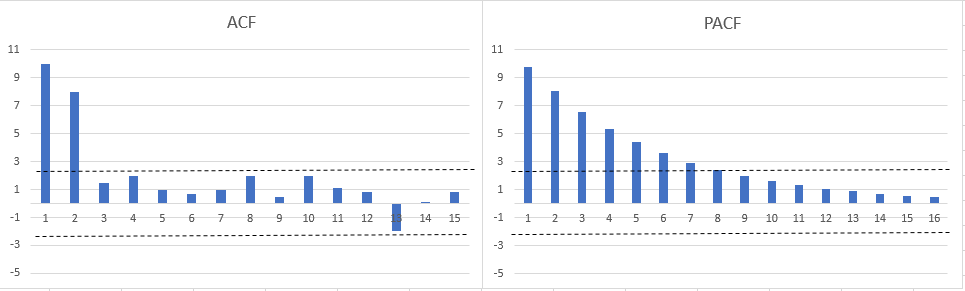
\includegraphics[width=16cm]{./acf-pacf.PNG}
\caption{グラフA}
\end{figure}

\begin{figure}[htbp]
\centering
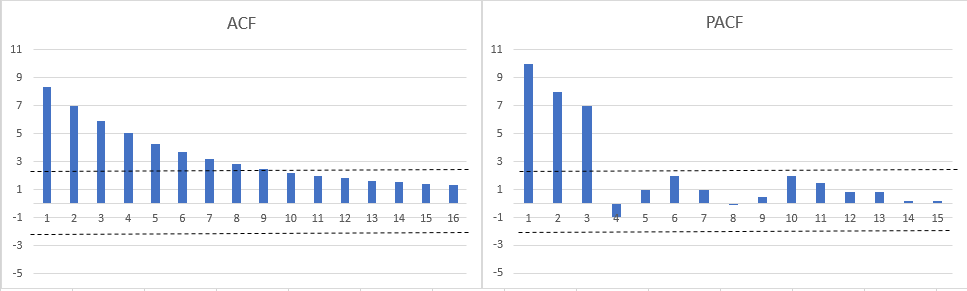
\includegraphics[width=16cm]{./pacf-acf.PNG}
\caption{グラフB}
\end{figure}

 簡潔に言うならば ACF と q、 PACF と p が強く関係している。\\
 グラフ A に着目すると、自己相関 の 1 次までの値が閾値を大きく超えていることがわかる。 自己相関 はラグkの共分散であり、偏自己相関 と違って 自己相関 はラグ k-1 やそれ未満の値の影響を考慮していない。よってノイズの重みを示している MA(q) モデルの、 q の値が決まると考えることができ、この例で言うならば \(q = 1\) であると考えることが出来る。\\
 同様にグラフ B に着目すると、偏自己相関 の 2 次までの値が閾値を大きく超えていることがわかる。偏自己相関 で説明したように、偏自己相関 の値は AR モデルに非常に近い形で用いることができ、このことから AR(p) モデルの p の値が決まると考えることができることがわかり、 \(p = 2\) がふさわしいことがわかるだろう。\footnote{詳しい証明について調べたものの、発見ができなかったため 引用を行ったサイト \cite{stat510} に書かれた内容を元に記述した}\\

 尚この p, q の値は観測者によって異なることがあるため、完全な正解があるわけではない。\\
 MA モデル (グラフA) における PACF 、 AR モデル(グラフB)における ACF のグラフは先細りの形を示している。これは上に示した 2 つのグラフが極めて理想的な MA / AR モデルを示していることを意味している。ARMA モデルの場合は ACF、PACF は共に先細りの形ではないため、この2つのグラフを見て係数 p, q を決定しなければならない。ところが AR モデルと MAモデルを同時に用いる場合、お互いの影響を打ち消し合ってしまう可能性があり、この係数決定は慎重に行わなければならない。ここで階差の次数 d も合わせた詳しい係数の決定基準と性質を以下に示す。\cite{acf-pacf} 尚 ここで用いる``カットオフ''とは、グラフAの ACF グラフにおける 0 \(\sim\) 2次の自己相関 から 3次の自己相関 への変化を意味する。\\
\begin{enumerate}
\item  その系列の 自己相関 が高い場合にはより高い階差を取る必要がある\\
\item  1 次の 自己相関 が0以下の場合、或いは 自己相関 がすべて小さくパターンが見られない場合には、それ以上の階差を取る必要はない\\
 1次の 自己相関 が -0.5 以下の値を取っているならば、階差を取りすぎている可能性がある\\
\item  階差の最もふさわしい次数は、多くの場合、標準偏差が最も低い階差の次数になる \footnote{これは階差は一般的には一次であるらしいという事実に反するが、階差が一般的に一次であるらしいという根拠が見つからなかったため検証を行うことができなかった}\\
\item  階差を取らない、つまり 0 次階差を取ることになった モデル は元の時系列データが定常であることを示している。\\
 1 次階差を取ることになったモデルは元の時系列データが何らかの傾向(ランダムウォークや Simple Exponential Smoothing type model\footnote{単純指数平滑法モデルとも言う})を持っていると考えられる。\\
 2 次階差を取ることになったモデルは元の時系列データが time-varying trend \footnote{翻訳が見つけることができなかったため意訳をすると、時間的変動傾向}(random trend や Linear Exponential Smoothing type model\footnote{Brownの線形指数平滑法モデルとも言う})を持っていると考えられる。\\
\item  階差を取らないモデルは通常定数項を持っている。2 次階差を持つモデルは通常定数項を持たない。\\
 1 次階差を取るモデルで、元の時系列が 0 でない傾きを持っているならば 定数項を考慮する必要がある。\\
\item  差分を取った時系列の PACF グラフが鋭いカットオフを示している場合、或いは更に 1 次の自己相関が正である場合にはモデルにARモデルを追加することを検討する必要がある。\\
 AR(p) モデルの p の値はカットオフを示している次数である。(グラフBならば \(p = 2\))\\
\item  差分を取った時系列の ACF グラフが鋭いカットオフを示している場合、或いは更に 1 次の自己相関が負である場合にはモデルにMAモデルを追加することを検討する必要がある。\\
 MA(q) モデルの q の値はカットオフを示している次数である。(グラフAならば \(q=1\))\\
\item  ARMA モデルが差分を取った時系列に適合する場合には p, q の値をそれぞれ 1 下げた場合のモデルを検証する必要がある。\\
 ARMA(p, q) ならば ARMA(p - 1, q) 、 ARMA(p, q - 1)\\
 特に ARMA モデルのパラメータ推定値が収束するために 10 回以上の 反復を必要とした場合にはこれを行うべきである。\\
\item  AR モデルに単位根が含まれている場合 \footnote{ARモデル部分のパラメータの合計値が大凡 1 であるとき} 、 p の値を 1 下げて階差の次数を 1 上げるべきである。\\
\item  MA モデルに単位根が含まれている場合 \footnote{MAモデル部分のパラメータの合計値が大凡 1 であるとき} 、 q の値を 1 下げて階差の次数を 1 下げるべきである。\\
\item  長期予測が奇妙な動きを見せている場合には、AR モデルか MA モデルに単位根が存在している可能性がある。\\
\end{enumerate}

\subsection{パラメータ推定}
\label{sec:org25b7e6f}
 ここまでにおいて ARIMA モデルの係数 p, d, q を決定することが出来る。ここから ARモデル、MAモデルそれぞれにおける、 \(\phi\) 、 \(\theta\) の値を推測する手法を説明する。このパラメータ推定は最尤推定(maximum likelihood)や CSS (conditional sum of squares) が用いられるようである。本演習では対数尤度関数に対してアメーバ法を適用してパラメータ推定を行った。これに際しアメーバ法の適用や、対数尤度関数の実装などについては Clojure for Data Science \cite{data-science} を活用した。\\
\subsubsection{対数尤度関数}
\label{sec:org2b68a9a}
 本演習では計算の都合上対数尤度関数を用いて最尤推定を行った。対数尤度関数に関しては既存のコードを読んで実装し、実装後に資料 \cite{log-likelihood} を用いて学習を行った。しかし理解が曖昧な部分が多いため本演習では詳細を示すことができなかった。\\
\subsubsection{アメーバ法}
\label{sec:orgebe5474}
 アメーバ法とは Nelder-Mead法とも呼ばれるパラメータ推定などに用いられる手法であり、本演習では対数尤度関数に対してこれを適用した。\\
 アメーバ法の特徴に目的となる関数の導関数が不要であることがある。これは本演習における対数尤度関数などの複雑な関数に対して有効なアルゴリズムである。アメーバ法の基本的なアルゴリズムは、反射、収縮、膨張の三種類であり、最適解の存在する位置に向かってアメーバのように近づいていくことからこの名前がついている。\\
 具体的な動きを二次元の図で表したものを引用 \cite{nelder-mead} すると以下のようになる。 \(Ti\) はアメーバの領域を示しており、これは議論の次元数に対して 1 つ多い頂点を持っている(この場合では 2次元に対して 3 頂点)。番号 \(i\) は動きの順番を示しており、反射\footnote{反転、或いは移動と考えることも出来る}、縮小を行いながら収束していることがわかる。拡大についてはこの図では見られない動きであるが、頂点を動かした先がより求めたい最大/最小に近いと判断できた場合に、そのまま頂点を引き伸ばす様を考えることができる。\\
 本演習では詳しいアルゴリズムの実装については調べず、ACM3に含まれている関数をそのまま用いた。\\
\begin{figure}[htbp]
\centering
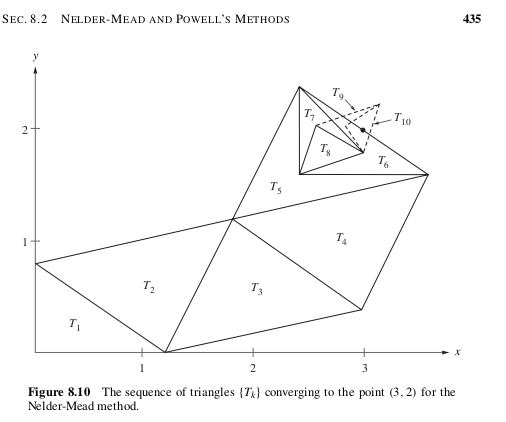
\includegraphics[width=15cm]{./nelder-mead.png}
\caption{アメーバ法の概略図}
\end{figure}

\subsubsection{AIC}
\label{sec:orgb3eb3c6}
 AIC (赤池情報量) はモデルの過適合などを判定するための指標であり、求めることができた対数尤度の適合度に対して p, q の値を考慮して計算される。具体的には以下の式を用いた。\\
\begin{align}
AIC = 2 * (p + q + 1) - 2 * log L
\end{align}
 尚 Lとは対数尤度である。AIC を最小化させることがモデルの適合度を上げることになる。\\
\subsection{SARIMA モデルについて}
\label{sec:orgf282bf4}
 本演習においては SARIMA (seasonal arima) モデルを作成することが目標であったが、現実のデータにおいて等間隔で周期を持ったものが少ないことが実装中に判明した。例えば、月単位のデータは1年周期(=12ヶ月周期)で階差を取ることが出来るが、週単位のデータは1年周期(\(=52.1429\))で階差を取ることができない。週単位のデータを近似的に1年周期で階差を取る、つまり数年ごとに調整を入れる案も考え実験をしたものの、予測を行った際における調整した分の補完が困難を極めたため実装を中断した。\\
 しかしながら季節階差を取る、という発想自体は間違いではない。具体的にどのような式に基づいて SARIMA モデルが作成されているかを \(SARIMA(1,1,1)(1,1,1)_{12}\) を用いて示す。尚説明の簡略化のため定数項は無視している。\footnote{SARIMA(非季節部分のパラメータp, d, q)(季節部分のパラメータP, D, Q){季節階差のラグ}}
\begin{align}
(1-\phi_1 B)(1-\phi'_1B^{12})(1-B)(1-B^{12})Y_t = (1+\theta_1B)(1+\theta'_1B^{12})\epsilon_t
\end{align}
\begin{itemize}
\item \((1-\phi_1 B)\) \\
 非季節部分のAR(1)モデルの項\\
\item \((1-\phi'_1B^{12})\)\\
 季節部分のAR(1)モデルの項\\
\item \((1-B)\)\\
 非季節部分の階差\\
\item \((1-B^{12})\)\\
 季節部分の階差\\
\item \((1+\theta_1B)\)\\
 非季節部分のMA(1)モデルの項\\
\item \((1+\theta'_1B^{12})\)\\
  季節部分のMA(1)モデルの項\\
この式からわかるように SARIMA モデルは ARIMA モデルに対して単純な乗算を行ったのみとなっている。これは ARIMA モデルのアプローチを大きく逸脱していないことを意味している。実際 ACF や PACF に関しては ARIMA モデルと同様に SARIMA モデルにもほとんど同じように適用することが出来る。\footnote{但し季節階差を取ったものに対して ACF/PACF を示した後、ARIMA モデルで用いた意味での ACF/PACF を適用していくという順番を負う}\\
\end{itemize}
\section{Clojure/ClojureScript を用いた Web 開発}
\label{sec:org5743b5e}
 本演習では開発言語として Clojure/ClojureScript を取り上げた。この 2 言語は Java/JavaScript をカバーした言語であるが、Java/JavaScript とは違い2つの言語に大きな差はない。またこの言語はWeb開発に適した言語であり、その WebSocket の質などは極めて優秀であるという比較\footnote{\href{https://hashrocket.com/blog/posts/websocket-shootout}{Websocket Shootout: Clojure, C++, Elixir, Go, NodeJS, and Ruby}} もある。更に Lisp であるという特性から HTML に代表されるマークアップ言語、SQLなどのドメイン特化言語を記述することが容易である。また \ref{sec:org9a4b90f} 先述のように高速計算も可能であることから ARIMA モデルに関するライブラリ作成、OpenTSDBへの接続、バックエンド、フロントエンドを実質一つのシンタックスで開発することができる。\\
 この章では実際にWeb開発で用いたライブラリなどを簡潔に示す。\\
\subsection{Clojure によるバックエンド開発}
\label{sec:orgb7533b6}
 バックエンド開発は \href{http://www.luminusweb.net/}{Luminus Framework} を用いて行った。その際 Web API としての動作を確認するために \href{https://swagger.io/swagger-ui/}{Swagger UI} を用いた。\\
\subsubsection{Luminus Framework}
\label{sec:orgdeb0a41}
 Luminus Framework とは Clojure の Web 開発に関するライブラリを統合したフレームワークである。ライブラリへのアクセスが極めて単純であり、それぞれのライブラリを好きなライブラリへ置換することも容易であるため、極めて自由度の高いフレームワークとなっている。そういった意味では Luminus はフレームワークと言うよりも推奨ライブラリのライブラリと言った方が近いのかも知れない。また様々なデータベースへのアクセスもサポート \footnote{OpenTSDBへの接続に関するサポートはなかったため、この部分の一部を自作する必要があった} されており、本演習ではSQLとして PostgreSQL を用いた。また Luminus には教科書とも言える書籍 \cite{luminus} があり、これをチュートリアルとして活用することが出来る。\\
\subsubsection{Swagger UI}
\label{sec:orgdf4b850}
 Swagger UI とは \href{https://swagger.io/tools/}{Swagger Tools} と呼ばれる RESTful API を作成するための支援ツール群の一つであり、ブラウザから API の動作を確認することが出来る。本演習では Swagger Tools の一部である Swagger UI のみを用いているが、これは \textcircled{\scriptsize 1} 関数型言語の特性の一つとして、データの源泉からデータの変換が終了するまでをひと続きに記述することが容易であるということから、サーバとクライアントのやり取りを行う部分のみを独立して記述することが効率的でないと判断したため \textcircled{\scriptsize 2} Clojure の REPL\footnote{Read-Eval-Print Loop 書いたコードを評価することでそれを反映することが出来る} 上で開発を行っているためブラウザからAPIの確認を行う以上の高機能を求めていないため \textcircled{\scriptsize 3} Luminus に含まれるライブラリである \href{https://github.com/metosin/compojure-api}{Compojure-api} のサンプルでは Swagger UI を API の確認以上の目的で使用していないためである。\\
 以下に実際に実装で用いた画面例を示す。\\
\begin{figure}[htbp]
\centering
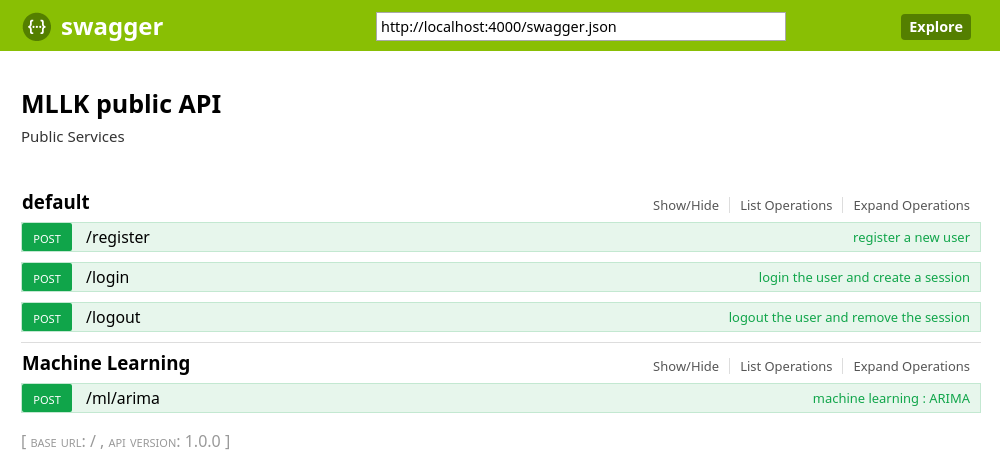
\includegraphics[width=15cm]{./swagger-ui-view.PNG}
\caption{Swagger UI の利用例\textcircled{\scriptsize 1}}
\end{figure}

 default という部分に含まれる POST メソッドは上から順に\textcircled{\scriptsize 1}ユーザ登録\textcircled{\scriptsize 2}ログイン認証\textcircled{\scriptsize 3}ログアウト、を意味している。これらの項目をクリックすることで必要なクエリやリクエストボディを入力することが出来る欄を開くことが出来る。開発者はここにテストとしてクエリを書き込むことでコードの妥当性を確かめることが出来る。\\

\begin{figure}[htbp]
\centering
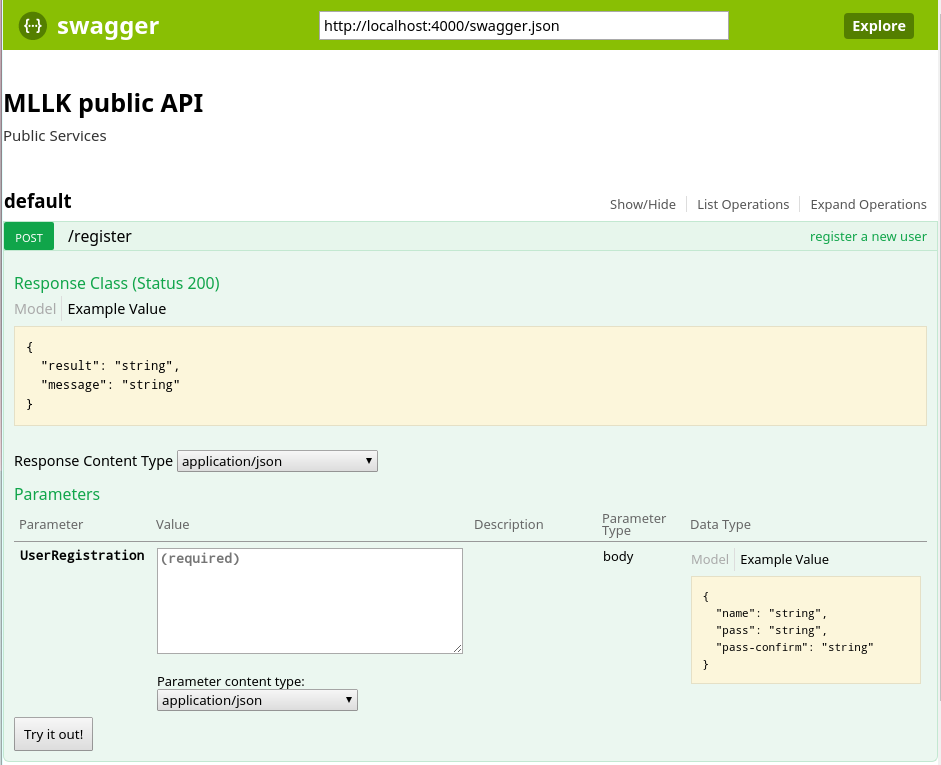
\includegraphics[width=15cm]{./swagger-ui-view2.PNG}
\caption{Swagger UI の利用例\textcircled{\scriptsize 2}}
\end{figure}
\newpage
\subsection{ClojureScript によるフロントエンド開発}
\label{sec:org7431a95}
 フロントエンド開発に関しては Luminus Framework ある機能に加え、 \href{https://reactjs.org/}{React.js} の ClojureScript ラッパーである \href{https://reagent-project.github.io/}{Reagent} 、React に特化された CSS フレームワークである \href{http://www.material-ui.com/\#/}{Material UI} を用いて作成した。\\
\subsubsection{基本的な開発}
\label{sec:orgb6fe603}
 Luminus Framework には Reagent を追加するオプションがあり、これを中心にフロントエンド側の開発を行った。またリクエスト処理などは Ajax を用いて実装した。\\
\subsubsection{Reagent}
\label{sec:org514ddf5}
 Reagent は React.js の ClojureScript ラッパーである。React.js とは UI を作成するための JavaScript ライブラリであり、ボタンやスライダーなどのコンポーネントを簡単に作成することが出来る。Reagent では HTML との連携を非常に簡単に行えるようになっており非常に見やすいシンタックスを提供する。以下に実際に実装に用いた例を紹介する。\\

\captionof{listing}{login-form関数}
\begin{minted}[frame=lines,linenos=true,obeytabs,tabsize=4]{clojure}
(defn login-form []
  (let [fields (atom {}) ;; 局所変数
        error (atom nil)] 
    (fn [] ;; 描画時に呼び出される無名関数として定義
      [c/modal ;; 自作関数であるモーダルウィンドウのコンポーネント呼び出し
       [:div "MLLK Login"] ;; モーダルのタイトル <div> 要素として記述
       [:div               ;; モーダルの内容
        [:div.well.well-sm ;; well well-sm は bootstrap のクラス
         [:strong "* required fields"]]
        [c/text-input "name" :name "enter a pass user name" fields] 
        ;; 自作のテキストフィールドの呼び出し
        (when-let [error- (:name @error)]
          [:div.alert.alert-danger error-]) ;; 名前に関するエラーを表示
        [c/password-input "password" :pass "enter a password" fields]
        (when-let [error- (:pass @error)]
          [:div.alert.alert-danger error-])
        (when-let [error- (:server-error @error)]
          [:div.alert.alert-danger error-])]
       [:div ;; <div><button type="button" class= "btn btn-primary" ...>
             ;;    ...</button><button ...>...</button><div>
        [:button.btn.btn-primary
         {:on-click #(login! fields error)} 
         ;; ボタンクリック時の動作を指定 (自作の関数 login! を呼び出している)
         "Login"]
        [:button.btn.btn-danger
         {:on-click #(session/remove! :modal)} 
         "Cancel"]]])))
\end{minted}

 一見すると非常に入り組んだ構造に見えるかも知れないが、それは HTML を記述している中に JavaScript を直接埋め込んでいるような記述をしているためである。しかし HTML と JavaScript をまとめて記述することで どこに何があるのか という疑問を持たずに済む。また細かいパーツに関数として分割することが出来るため \footnote{正確には関数が評価されるタイミングを考慮する必要がある} 、 上例のように ログインフォームのみを独立して記述をすれば、 全体として大きな構造が必要となったとしても小さな構造体に問題を分割することが出来る。\\
 以下がこのソースコードを中心にして作成された login-form である。\\
\begin{figure}[htbp]
\centering
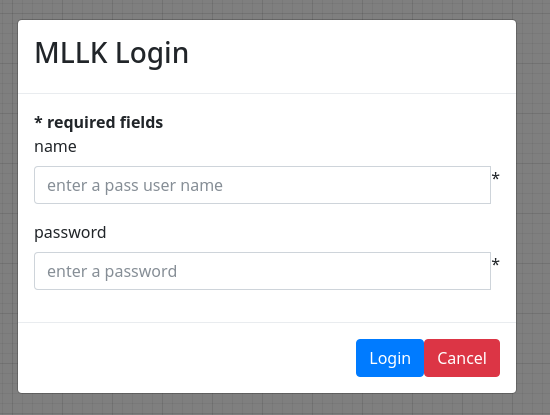
\includegraphics[width=15cm]{./login-view.PNG}
\caption{login-form}
\end{figure}

\section{MLLK の開発}
\label{sec:orgd2d0c53}
 本演習では紆余曲折があったものの最終的には MLLK (Machine Learning Learning Kit) という Web アプリケーションのベータ版を開発した。完成まで導くことができなかった原因は、公開に足る性能を達成できなかったこと、アプリケーションの安全性が確立できなかったこと、データベースサーバなどの環境が特別であったため公開可能なサーバを調達できなかったことである。\\
\subsection{ARIMA モデルライブラリ}
\label{sec:org82b97e7}
  \ref{sec:org73bc3ce} ARIMA モデルによる時系列分析 に従ってそれぞれの関数を実装した。\\
\subsection{データベース設計}
\label{sec:org0cfdbf3}
 以下の図に従ってデータベースを作成した。以降にそれぞれのテーブルについて説明する。\\
\begin{figure}[htbp]
\centering
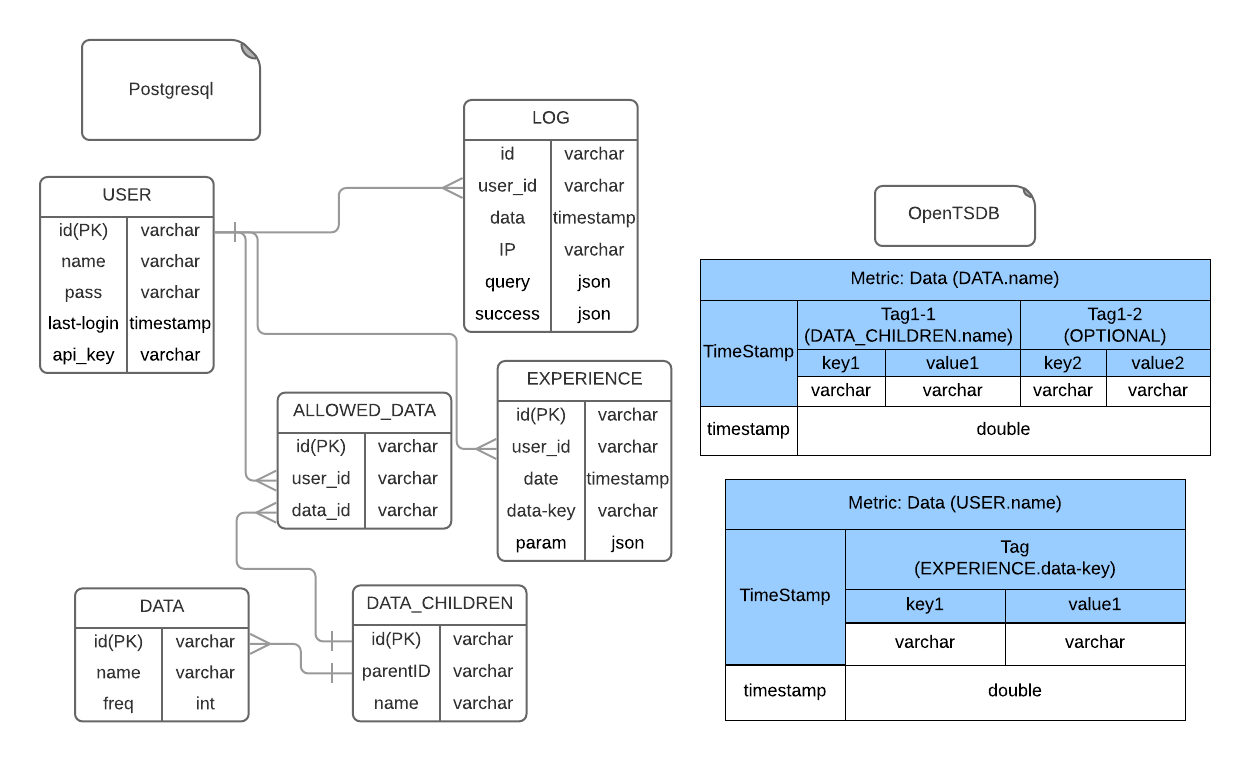
\includegraphics[width=15cm]{./fool-diagram.png}
\caption{データベースの設計図}
\end{figure}
\subsubsection{Postgresql}
\label{sec:org43d12cf}
 SQL サーバとしては \href{https://www.postgresql.org/}{Postgresql} を採用した。\\
\begin{itemize}
\item USERS\\
 ユーザに関するデータを保存している。name はユーザの名前、pass は暗号化済みのパスワード、last\_login は最後のログイン時間、 api\_key は ユーザが持つ Quandl のAPIキーである。admin は管理者権限で本演習ではすべてのユーザが偽にセットされている。id は主キーであり、これは他のテーブルにも共通している。\\
\item LOG\\
 ユーザが行った情報をまとめるためのテーブルであるが、今回は実際にテーブルの作成のみで実際にテーブルを動かすことはできなかった。query と success はログインなどのクエリと対応付けられた 番号 が、 date にはそのクエリが送られた日時が当てはまる。IP にはユーザがアクセスした端末の IP アドレスが当てはまる。\\
\item TSDATA\\
 例えば ``NIKKEI/INDEX'' のような時系列データの名称を保存するためのテーブルである。name はその時系列データの名前である。freq はデータの時間的頻度を指定しているが、ARIMA モデルの規格化などもあり今回はすべて週ごとを示す ``weekly'' がセットされている。\\
\item TSDATA\_CHILDREN\\
 ``close-price'' のような TSDATA テーブル で扱うべきではない細かいデータ区分を保存するためのテーブルである。name はその区分を示す名前である。ここにある name と parent\_name を用いて OpenTSDB の Metric TSData に保存された時系列データへのアクセスを行う。\footnote{TSDATAの Metric 名は TSDATAテーブルの name , タグの value が TSDATA\_CHILDREN テーブルの name に対応している}\\
\item ALLOWED\_DATA\\
 ユーザごとに扱えるデータに制限をかけるためのテーブルである。これは Quandl がAPIキーを登録せずともある上限まではデータを入手できるという機能に即するために作成した。\\
\item EXPERIENCE\\
 ユーザの実験データを保存するが、本演習では機能の実装が完了できなかったためテーブルのみの実装になった。 date は実行日時、data\_key は OpenTSDB の Metric EXData にある タグの value の値である。 param には行った機械学習の種類やパラメータが含まれた JSON が当てはまる。\\
\end{itemize}
\subsubsection{OpenTSDB}
\label{sec:org29139dc}
 時系列データに関しては \ref{sec:org73bc3ce} ARIMA モデルによる時系列分析 にあるとおり、 OpenTSDB を用いた。\\
\begin{itemize}
\item TSData\\
 実際の時系列データを保存するためのデータベースである。本演習ではデータの入手元は \href{https://www.quandl.com/}{Quandl.com} のみであった。Metrics には ``NIKKEI/INDEX'' のような 時系列データの名称が当てはまり、タグの key は本演習では混乱を避けるために ``type'' に統一されており、そしてタグの value は ``close-price'' などの時系列データ内のカテゴリが当てはめられている。\\
\item EXData\\
 本演習では実装が終わらず実際に稼働させることはできなかった。Metric には Postgresql にある USERS テーブルの name が当てはまり、タグの key には ``key'' が、 value には Postgresql の EXPERIENCE の data\_key が当てはまる。\\
\end{itemize}

\subsection{バックエンド開発}
\label{sec:orgb2023a0}
 バックエンドは \ref{sec:org5743b5e} にあるように、 Luminus Framework を中心に開発を行った。作成した ARIMA モデル やそれに関するライブラリや OpenTSDB を用いるための簡易的なAPI などは別個依存関係に加えた。フロントエンドも含めた\footnote{バックエンドとフロントエンドは同一のプロジェクトとして作成されている}具体的な依存関係は 開発を行っている git@github:MokkeMeguru/MLLK にある \href{https://github.com/MokkeMeguru/MLLK/blob/master/project.clj}{project.clj} にある。\\
\subsection{フロントエンド開発}
\label{sec:orgcc0a17e}
 フロントエンドの開発もバックエンド同様 Luminus を用いて行った。以下に実際の画面をユーザが利用する場面を想定して説明する。\\
 まずユーザはホームページにアクセスし、ユーザ登録画面へと遷移する。\\
\begin{figure}[htbp]
\centering
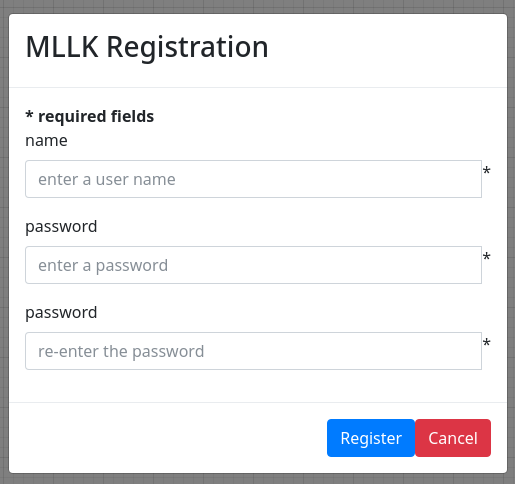
\includegraphics[width=8cm]{./register.PNG}
\caption{ユーザ登録画面}
\end{figure}

 或いは既にユーザ登録が済んでいるユーザは名前とパスワードを入力しログインすることが出来る。この画面は既に \ref{sec:org7431a95} ClojureScript によるフロントエンド開発 で紹介済みであるため省略する。\\
\newpage
 次にユーザは実際に ARIMA モデルを (或いは開発が終了した場合にはそれらの手法を) 実行するためにこれらを行う画面へ遷移する。\\
\begin{figure}[htbp]
\centering
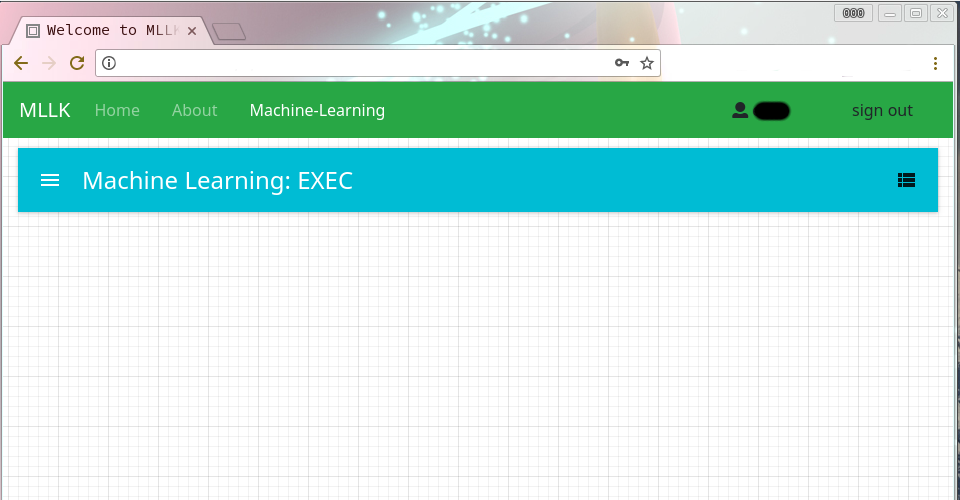
\includegraphics[width=12cm]{./ml-view.PNG}
\caption{統計・機械学習手法選択画面}
\end{figure}

 ここで機械学習手法を青枠右側にあるメニューアイコンから呼び出し選択を行う。次に青枠左側にあるメニューアイコンを選択すると以下のようになる。\\

\begin{figure}[htbp]
\centering
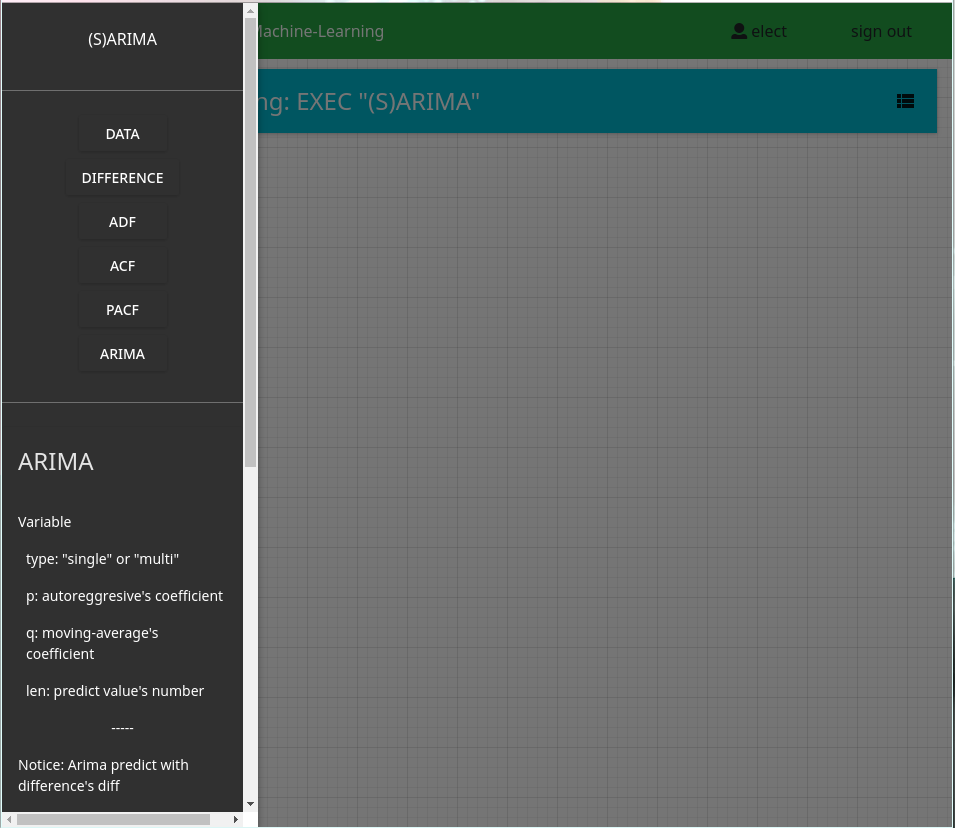
\includegraphics[width=12cm]{./settings-view.PNG}
\caption{パラメータ設定画面}
\end{figure}
\newpage
 パラメータを選択する画面である。上にある``DATA''などと書かれているボタンはそれぞれのパラメータを入力する画面へ遷移する (現在は``ARIMA''ボタンを選択した状態)。はじめに大まかな説明がつき、その下に詳しい説明へのリンク (正確な理論が書き上がり次第組み込まれる) 、そしてパラメータの入力欄が続いていく。ユーザはこれらの必要な項目の入力が済ませ実行ボタンである``run''ボタンを押す。\\

\begin{figure}[htbp]
\centering
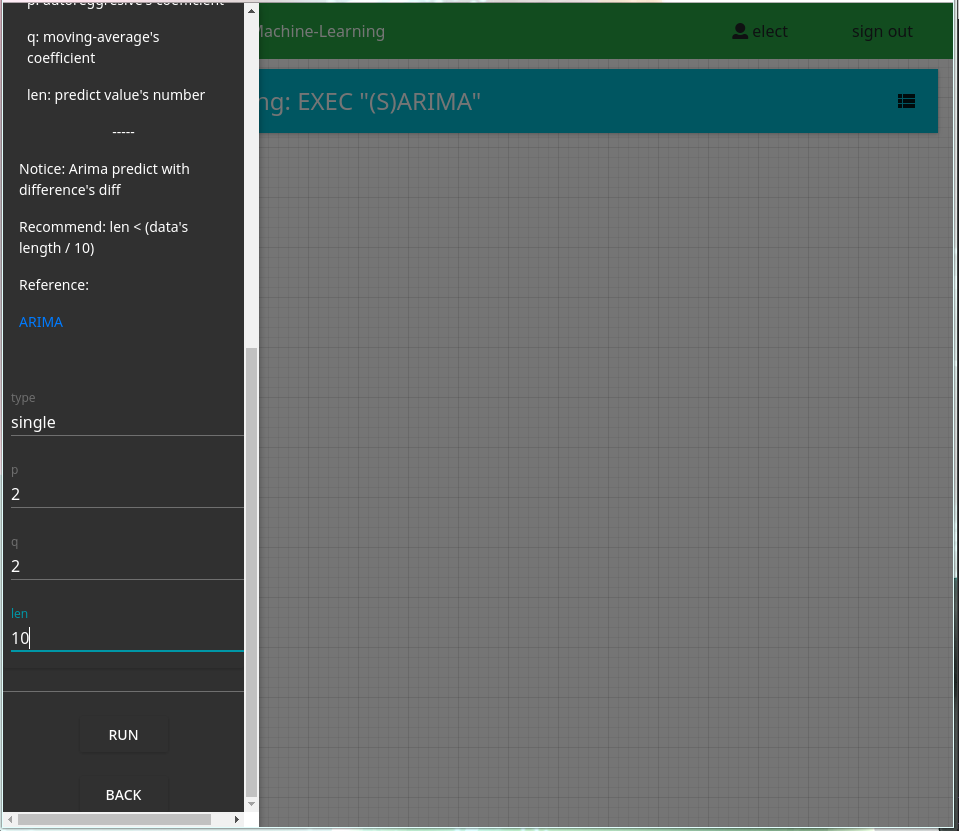
\includegraphics[width=.9\linewidth]{./settings-view2.PNG}
\caption{パラメータ入力欄と実行ボタン、説明ページへのリンク}
\end{figure}

  実行することでユーザは以下のような画面を得る。\\
\begin{figure}[htbp]
\centering
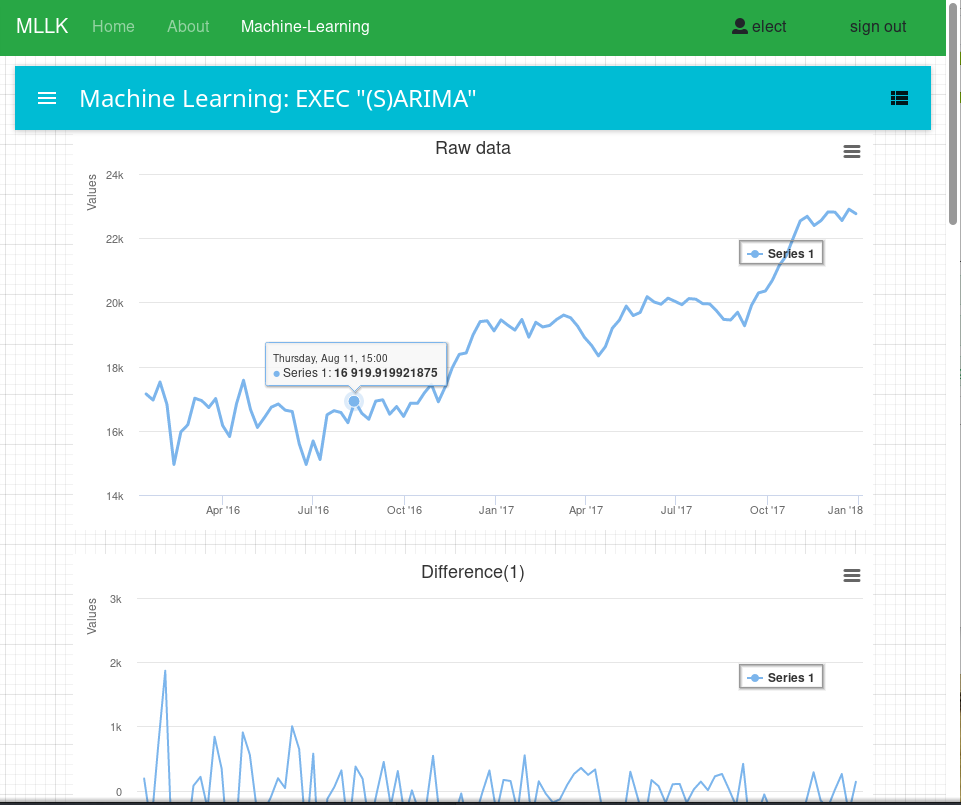
\includegraphics[width=10cm]{./arima-view.PNG}
\caption{実行結果画面}
\end{figure}

  尚 2018年1月18日時点 で出力可能な内容を印刷した pdf を \ref{sec:orgf55781c} 付録に追記する。\\
\newpage
\section{ARIMA 推定 と Random Forest による予測}
\label{sec:org26d20d0}
 この章では \ref{sec:org5388bcc} 序論で言及した (S)ARIMA モデルを用いた時系列データ予測と Random Forest を用いた欠損値補完を組み合わせた手法の検証実験について示す。\\
\subsection{概要}
\label{sec:orga756cba}

 ARIMA 推定は 単一の時系列データに対してモデル推定・予測を行うが、これにある 予測 を 他のデータと関連させて行う 、という立場から予測を行いたいと考えた。つまりこの実験の目的は複数の時系列データに対して、 相関 を使って予測を行うというアプローチの妥当性について調査したい、ということである。\\

\subsection{実験方法}
\label{sec:orgc221c42}
  \href{https://github.com/millejoh/emacs-ipython-notebook}{Emacs IPython Notebook} を用いて Python の既存である関数を用いて実験を行う。\\
 実験データは Quandl から入手し、使用するデータは \textcircled{\scriptsize 1} 日経平均株価 \textcircled{\scriptsize 2} アサヒグループホールディングス \textcircled{\scriptsize 3} JR 東日本 \textcircled{\scriptsize 4} トヨタ自動車 \textcircled{\scriptsize 5} アステラス製薬 \textcircled{\scriptsize 6} ソニー の6つの終値である。\\
 実験手順は 以下のとおりである。\\
\newpage
\begin{enumerate}
\item \textcircled{\scriptsize 2} から \textcircled{\scriptsize 6} の 2015年1月 から 2017年4月 までの 週次 データに対して ARIMA モデルを適用し、2017年11月頭までの予測を行う。\\
\item \textcircled{\scriptsize 1} から \textcircled{\scriptsize 6} における 2015年1月 から 2017年4月 までの時系列データに対して Random Forest を用いて回帰分析を行う。\\
 目的変数は \textcircled{\scriptsize 1} であり、説明変数は \textcircled{\scriptsize 2} から \textcircled{\scriptsize 6} である。\\
\item 得られた Random Forest のモデルを用いて \textcircled{\scriptsize 1} について2017年11月頭までの予測を行う。\\
\item 実際の \textcircled{\scriptsize 1} の値と比較を行う。\\
\item Random Forest のみによる回帰分析、ARIMA モデル、 SARIMA モデルのそれぞれを \textcircled{\scriptsize 1} に適用し、 3. と精度比較を行う。\\
\end{enumerate}
\subsection{実験結果}
\label{sec:org8902258}
 膨大な実験データになったため、付録に解説を含めて添付する。\\
\subsection{考察}
\label{sec:orgf96ec5c}
 提案した手法は実験結果からわかるように良い精度を得られなかった。原因として考えられるものに、ARIMAモデルそのものが精度を必ずしも保証できないということ、説明変数の選択が不適切であったことが考えられる。\\
 実際に実験中に用いた ARIMA モデルは予測精度に難があり、SARIMA モデルを使わなければならなかった。そしてその判定は AIC 等を用いて求める他に、それぞれの実行結果を目で確認する必要があるのではないかと考えている。季節階差などは ACF や PACF のグラフの閾値内にも隠れている可能性が十分にあることは今回の実験から明らかである。\\
 説明変数の選択については、この実験は複数回実行されておりぞれぞれ 4 \(\sim\) 5 個の説明変数を用いて行ったものの、この実験結果とほとんど変わらない精度であったことから、非常に難しい問題であると考えている。特に株価のような様々な要因が複雑に重なり合って初めて決定されると考えられるデータに対して最適な説明変数を選択することは、相当に株式について知見を持った観測者でなければ出来ないと考えている。但し、例えば仮想的に小さな世界を作成し、その中でのみ相互作用が起こる場合にこの手法を適用した場合にどのような結果が出るのか、という疑問が生まれた。この検証については今演習では時間や能力が足りず実験を行うことが出来なかったため、来年度以降の課題としたい。\\
\section{まとめと今後の課題}
\label{sec:org0f59b9f}
 本演習で学んだ内容は非常に多岐に渡っており、来年度以降の研究題材を豊富に得ることができたと考えている。\\
 例えば本演習中に GPU 計算について学ぶ際に GPU を用いた開発の花形の一つとも言えるゲームエンジン・グラフィックエンジンの開発について触れる場面があった。現在一部のゲームを除いて殆どのゲームは C++ をベースに作成されているが、JVM 言語も GPU を用いた高速計算が可能である。このため Clojure を用いて高速なゲームエンジンを作成してみる、更にはそこに何かしらのゲームAIを組み込んでみる、ということは需要については議論の余地があるとしても非常に興味深い内容になると考えている。\\
 また機械学習について調べていく途中で RNN \footnote{Reccurent Neural Network} を見る機会、黒板アーキテクチャ、当然のことながら Random Forest について学ぶ機会があり、様々な特徴を持ったデータベースについて触れる機会も得たため、これらを組み合わせてみた場合にどのようなことが出来るのかを検討・調査してみたいと考えている。\\
  本年度の情報特別演習はこなさなければならない課題は多かったが、その分学ぶ部分も多く存在した。残念でならない点は、量が増えたためかそれぞれの成果がやや雑に纏まってしまったということである。来年度は本年度以上に課題を多く解くと共に、その課題一つ一つに真摯に取り組んでいこうと考えている。\\

\section{謝辞}
\label{sec:orgab0062c}
 本演習においてはグループメンバーや担当教員である 筑波大学 システム情報系 情報工学域 日野 英逸 准教授に多大なご指導を頂いた。具体的には、グループメンバーには様々な課題を賜り充実した演習を行うことが出来、准教授には実験のみならずレポートの作成などについてもご指導を頂いた。協力に心からの感謝を申し上げます。
\newpage
\section{付録}
\label{sec:orgf55781c}
\subsection{このレポートにおける数式について}
\label{sec:orgc97f0cc}
 このレポートにおける数式表現といくつかの基本的な用語の定義を以下に例と共に示す。\\
\subsubsection{独立同時分布と変数の補足}
\label{sec:org6fbf02b}
\begin{align}
Y_t = \beta t + \epsilon_t \ where \ \epsilon_t \sim iid(0, \sigma^2)
\end{align}
 この式における \(where\) とは左式における変数の補足を行うことを意味しており、この場合で \(\epsilon_t\) の意味を補足している。\(iid(\mu, \sigma^2)\) とは 独立同時分布 (independent and identically distributed) を意味しており、この確率変数は他の確率変数と同一の分布を持ち、且つそれぞれが独立していることを示している。独立同時分布において共分散、相関係数は 0 である。本レポートにおいてこの式は、平均 \(\mu\) 、 分散 \(\sigma^2\) に従う \footnote{$a \sim b$ とは、 a は b という分布に従う という意味である} 独立同時分布という意味を持っている。\\
 これと同様の概念にホワイトノイズというものがあるため、混乱を避けるためこちらも補足を行う。\\
 ホワイトノイズ \(\epsilon_t \sim W.N(0, \sigma^2)\) は以下の性質を持っている。\\
\begin{itemize}
\item \(E(E_t) = 0\) \\
 平均は0\\
\item \(Var(E_t) < infinity\) \\
 分散は発散しない\\
\item \(Cor(E_t, E_s) = 0\) \\
 相関 (correlation) 関係はない \footnote{$r_{e_t, e_s}$ と表されることもある} \\
\end{itemize}
 ホワイトノイズと独立同時分布の関係は、ホワイトノイズには必ずしも独立性があるわけではないという意味で、独立同時分布のほうがより``強固''であると言える。 \\
\newpage
\subsubsection{標準誤差}
\label{sec:orgd168f56}
\begin{align}
\hat{\pi}/ se(\hat{\pi})
\end{align}
 この式における \(se(\hat{\pi})\) とは \(\hat{\pi}\) についての標準誤差を示している。ここで用いる標準誤差とは最小二乗法で求められる解ベクトル \(\hat{\beta}\) の要素 \(\hat{\beta_i} = \hat{\pi}\) についての誤差、最小二乗推定量 \(\hat{\beta_i}\) に関する標準誤差である。これは回帰の標準誤差とは異なることに注意しなければならない。以下に回帰に関する標準誤差を示し、その後最小二乗推定量 \(\hat{\beta_i}\) に関する標準誤差を示す。\\
 例として以下の式を真のモデルとする。但し \(u\) は誤差項であり、平均 \(0\) 分散 \(\sigma^2\) である独立同時分布に従う要素を持つベクトルであるとする。\footnote{X, $\beta$に定数項は含まれているものとする}\\
\begin{align}
\bm{y} &= \bm{X} \hat{\beta} + \bm{u} \nonumber \\
       &\ where \ \bm{y},\  \bm{u}\ is \ n * 1 \ vector  \nonumber \\
       &\ \ \ \ \ \ X\ is\ n * p\ matrix \nonumber \\
       &\ \ \ \ \ \ \bm{\beta}\ is\ p * 1\ vector \nonumber \\
       &\ \ \ \ \ \ \bm{u}\ \sim \ iid(0, \sigma^2 \bm{I}) \nonumber \\
       &\ \ \ \ \ \ \bm{I}\ is \ n * n \ identity\ matrix
\end{align}

 推定量 \(\hat{\beta}\) について求まる残差 \(\bm{\epsilon}\) は以下のように表すことが出来る。\\
\begin{align}
\bm{\epsilon} = \bm{y} - \bm{X}\hat{\beta}
\end{align}
 これを用いて残差平方和 SSR\footnote{sum of squared residuals} は、\\
\begin{align}
SSR &= \bm{\epsilon}' \bm{\epsilon} \nonumber \\
    &= \bm{y}' \bm{y} - 2 \beta' \bm{X}'y + \beta'\bm{X}'X\beta
\end{align}
 と表すことが出来る。これを用いて回帰の標準誤差\footnote{standard error of regression}は、\\
\begin{align}
s^2  = SSR / (n - p)
\end{align}
 となる。さらにこれを用いることで、最小二乗推定量 \(\hat{\beta_i}\) に関する標準誤差は、\\
\begin{align}
s.e.(\hat{\beta_i}) &= \sqrt{s^2/S_{XX}^j} \nonumber \\
&where\ S_{xx}^j = ((X'X)^{-1})_{jj}
\end{align}
 となる。尚 \(S_{xx}^j\) とは \(x_j\) から他の変数の影響を取り除いた \(x_j\) に固有の平方和である。\\

\subsection{出力結果}
\label{sec:orgd215215}
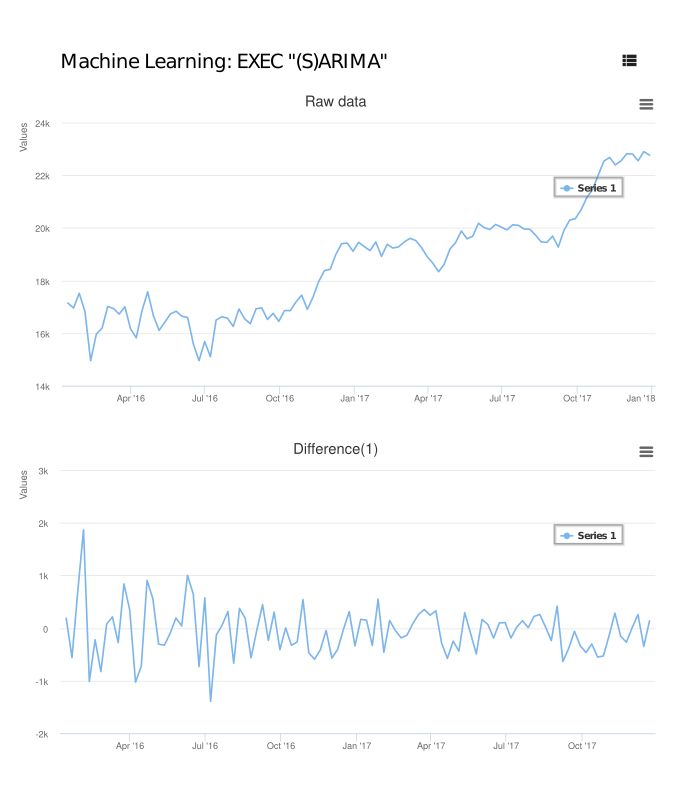
\includegraphics [width=16cm] {./rect4145.png}
\newpage
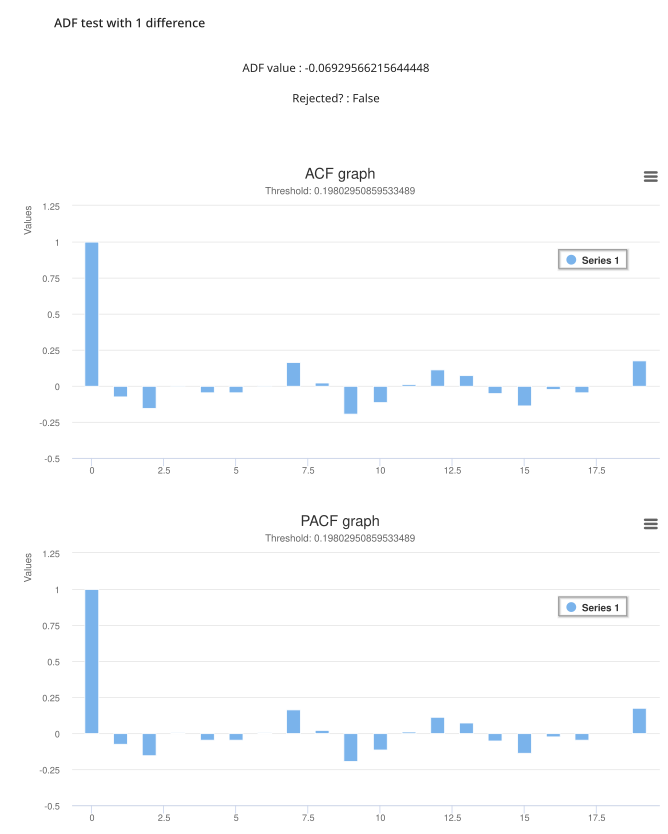
\includegraphics [width=16cm] {./rect1607.png}
\newpage
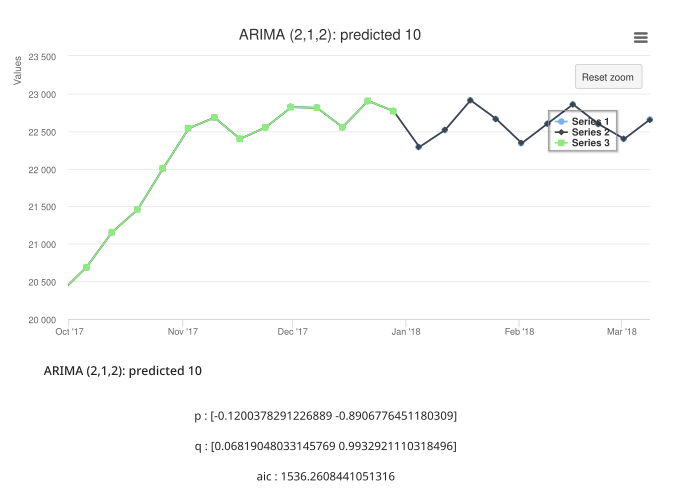
\includegraphics [width=16cm] {./rect1673.png}
 黒線とやや隠れてしまっているが青線の間がモンテカルロ法によって求めた\footnote{モデルのシミュレートを1000回行い、平均と標準偏差を求めている}予測の95\%信頼区間である。\\
\newpage

\subsection{実験結果}
\label{sec:org4f2ffe7}
 まず依存環境を解決する。\\
\begin{minted}[frame=lines,linenos=true,obeytabs,tabsize=4]{python}
from pprint import pprint
import warnings
warnings.filterwarnings('ignore')
import numpy as np
import pandas as pd
from scipy import stats
import quandl
from sklearn.ensemble import RandomForestRegressor
import statsmodels.api as sm
from statsmodels.tsa.arima_model import ARIMA, ARMA
from matplotlib import pylab as plt

%matplotlib inline
\end{minted}

 次に、データを入手するための関数を定義する。データは 2015年1月から2017年11月頭までの週次のものである。\\
\begin{minted}[frame=lines,linenos=true,obeytabs,tabsize=4]{python}
def get_dataframe (name) :
    return quandl.get(name, start_date='2015-1-1', end_date='2017-11-1',
                      collapse='weekly')
\end{minted}

 これを用いてデータを入手する。dataframe の後ろにつく数字は、 \ref{sec:orgc221c42} 実験方法に記載されている数字と一致している。\\
\begin{minted}[frame=lines,linenos=true,obeytabs,tabsize=4]{python}
dataframe1 = get_dataframe("NIKKEI/INDEX.4")
dataframe2 = get_dataframe("TSE/2502.4")
dataframe3 = get_dataframe("TSE/9020.4")
dataframe4 = get_dataframe("TSE/7203.4")
dataframe5 = get_dataframe("TSE/4503.4")
dataframe6 = get_dataframe("TSE/6758.4")
\end{minted}

 以下は入手したデータの整形である。\\
\begin{minted}[frame=lines,linenos=true,obeytabs,tabsize=4]{python}
ts1 = dataframe1['Close Price'].rename('Close')
ts2 = dataframe2['Close'][:120]
ts3 = dataframe3['Close'][:120]
ts4 = dataframe4['Close'][:120]
ts5 = dataframe5['Close'][:120]
ts6 = dataframe6['Close'][:120]
\end{minted}

 以降は ADF 検定を用いた定常性判定であり、最小となる階差の次数における分析結果が返される。返り値の 1 つめの要素と最後の Map の中身の値を比較して仮説検定が行われ、その際に用いられる次数、つまり最もふさわしい次数が 3 つめの要素である。今回は最も ADF の値が小さくなるように、定数と傾きに関する項を回帰に含めている。\\
\begin{minted}[frame=lines,linenos=true,obeytabs,tabsize=4]{python}
pprint(sm.tsa.stattools.adfuller(ts2, regression='ctt', autolag = 'AIC'))
pprint(sm.tsa.stattools.adfuller(ts3, regression='ct', autolag = 'AIC'))
pprint(sm.tsa.stattools.adfuller(ts4, regression='ctt', autolag = 'AIC'))
pprint(sm.tsa.stattools.adfuller(ts5, regression='ct', autolag = 'AIC'))
pprint(sm.tsa.stattools.adfuller(ts6, regression='ctt', autolag = 'AIC'))
\end{minted}

\begin{verbatim}
(-3.4243993894646616,
 0.13326170365782197,
 0,
 119,
 {'1%': -4.471237472469957,
  '10%': -3.584424431130831,
  '5%': -3.882969922547368},
 1307.5889250985836)
(-2.904793565308496,
 0.16067015581233307,
 0,
 119,
 {'1%': -4.036933565633866,
  '10%': -3.1490681814297643,
  '5%': -3.4480491338265407},
 1537.811468467928)
(-2.6037424086219305,
 0.5096036701299048,
 0,
 119,
 {'1%': -4.471237472469957,
  '10%': -3.584424431130831,
  '5%': -3.882969922547368},
 1449.4672932660785)
(-3.4174043810519117,
 0.04910564863187634,
 0,
 119,
 {'1%': -4.036933565633866,
  '10%': -3.1490681814297643,
  '5%': -3.4480491338265407},
 1143.8350636832258)
(-4.137776413232316,
 0.02100681603520161,
 1,
 118,
 {'1%': -4.472110860871852,
  '10%': -3.584692378310343,
  '5%': -3.883407308731662},
 1337.068933005826)
\end{verbatim}

 次に \textcircled{\scriptsize 2} から \textcircled{\scriptsize 6} の ARIMA モデルの係数 p, q の値を、Python の関数を用いて半自動的に求める。\\
\begin{minted}[frame=lines,linenos=true,obeytabs,tabsize=4]{python}
pprint(sm.tsa.arma_order_select_ic(ts2, ic='aic'))
pprint(sm.tsa.arma_order_select_ic(ts3, ic='aic'))
pprint(sm.tsa.arma_order_select_ic(ts4, ic='aic'))
pprint(sm.tsa.arma_order_select_ic(ts5, ic='aic'))
pprint(sm.tsa.arma_order_select_ic((ts6 - ts6.shift(1)).dropna(), ic='aic'))
\end{minted}

\begin{verbatim}
{'aic':              0            1            2
0  1679.536657  1577.743635  1763.332522
1  1488.936634  1490.614433  1488.660757
2  1490.733981  1490.708809  1490.657758
3  1489.374765  1491.192556  1492.459610
4  1491.350072  1493.041001  1494.459551,
 'aic_min_order': (1, 2)}
{'aic':              0            1            2
0  1979.585644  1869.081432  1809.600127
1  1737.428598  1738.866964  1739.981652
2  1738.990991  1740.494877  1741.980017
3  1739.657859  1741.646606  1735.021824
4  1741.609854  1743.301390          NaN,
 'aic_min_order': (3, 2)}
{'aic':              0            1            2
0  2002.003998  1868.465319  1964.683360
1  1640.157010  1641.641261  1643.141242
2  1641.711249  1642.628899  1644.606973
3  1643.150901  1644.607821  1647.420408
4  1645.148941  1646.595370  1648.894668,
 'aic_min_order': (1, 0)}
{'aic':              0            1            2
0  1545.805878  1436.081643  1388.521781
1  1302.593986  1303.591920  1304.847993
2  1303.801149  1305.297028  1306.731610
3  1304.443329  1306.432100  1292.806527
4  1306.403755  1310.297566  1294.654617,
 'aic_min_order': (3, 2)}
{'aic':              0            1            2
0  1525.435271  1522.249768  1523.248768
1  1521.388158  1522.796172  1524.758002
2  1522.815016  1524.769149          NaN
3  1524.725640  1526.723993          NaN
4  1526.710486  1528.435723          NaN,
 'aic_min_order': (1, 0)}
\end{verbatim}

 ここまでで ARIMA モデルにおける p, d, q の係数が定まったため、それらを適用してモデルを作成する。 尚 階差 d が 0 である場合は、この条件においては同義となる ARMA モデルを適用している。\\
\begin{minted}[frame=lines,linenos=true,obeytabs,tabsize=4]{python}
ts2_arima = ARMA(ts2, order = (1, 2)).fit()
ts3_arima = ARMA(ts3, order = (3, 2)).fit()
ts4_arima = ARMA(ts4, order = (1, 0)).fit()
ts5_arima = ARMA(ts5, order = (3, 2)).fit()
ts6_arima = ARIMA(ts6, order = (1, 1, 0)).fit()
\end{minted}

 次に Random Forest モデルを作成する。目的変数を\\
\begin{minted}[frame=lines,linenos=true,obeytabs,tabsize=4]{python}
  r_forest = RandomForestRegressor(n_estimators = 1000, criterion = 'mse',
                                   random_state = 1, n_jobs = 1)
r_forest.fit(np.vstack((ts2.values,ts3.values,ts4.values,ts5.values,ts6.values)).T,
             ts1[:120].values)
\end{minted}

 Random Forestのモデルを作成したので、 ARIMA モデルを適用した \textcircled{\scriptsize 2} から \textcircled{\scriptsize 6} を用いて予測値を作成する。\\
\begin{minted}[frame=lines,linenos=true,obeytabs,tabsize=4]{python}
ts2_predict = ts2_arima.predict('2015-1-18','2017-11-5')
ts3_predict = ts3_arima.predict('2015-1-18','2017-11-5')
ts4_predict = ts4_arima.predict('2015-1-18','2017-11-5')
ts5_predict = ts5_arima.predict('2015-1-18','2017-11-5')
ts6_predict = ts6_arima.predict('2015-1-18','2017-11-5')
\end{minted}

 必要な要素が揃ったため、ここで問題となる回帰予測をおこなった。\\
\begin{minted}[frame=lines,linenos=true,obeytabs,tabsize=4]{python}
ts1_pred_with_RF = r_forest.predict(
    np.vstack((ts2_predict, ts3_predict, ts4_predict, ts5_predict, ts6_predict)).T)
ts1_pred_with_RF_dataframe = \
pd.DataFrame({'Close': ts1_pred_with_RF.tolist()},index = \
    pd.DatetimeIndex(periods = 147, freq = 'W', start = '2015-1-18'))
plt.hold(True)
plt.plot(ts1_pred_with_RF_dataframe)
plt.plot(ts1)
\end{minted}

%\begin{verbatim}
%[<matplotlib.lines.Line2D at 0x7fbda6504400>]
%\end{verbatim}
\begin{center}
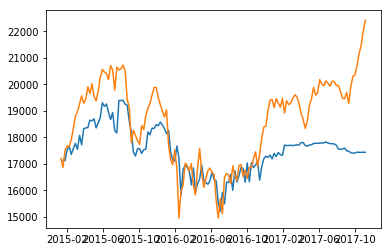
\includegraphics[width=.9\linewidth]{./obipy-resources/MOXXjm.png}
\end{center}

 この図を見るとこの手法はあまり精度が出ていないことがわかる。\\
 次に比較として、単純に \textcircled{\scriptsize 1} に ARIMA モデルを適用した場合の時系列予測を行う。行っていることは \textcircled{\scriptsize 2} 等と変わらないため解説は省く。\\
\begin{minted}[frame=lines,linenos=true,obeytabs,tabsize=4]{python}
sm.tsa.stattools.adfuller(ts1[:120], regression='ctt', autolag = 'AIC')
\end{minted}

\begin{verbatim}
(-2.8812138487142485,
0.3547039460728244,
0,
119,
{'1%': -4.471237472469957,
'10%': -3.584424431130831,
'5%': -3.882969922547368},
1624.5165654066914)
\end{verbatim}

\begin{minted}[frame=lines,linenos=true,obeytabs,tabsize=4]{python}
sm.tsa.arma_order_select_ic(ts1[:120], ic='aic')
\end{minted}

\begin{verbatim}
{'aic':              0            1            2
0  2096.943059  1986.989400  1930.176824
1  1837.682455  1839.576223  1841.481132
2  1839.583519  1841.552211  1843.455817
3  1841.446417  1843.432328  1843.027764
4  1843.368379          NaN  1845.121876, 'aic_min_order': (1, 0)}
\end{verbatim}

\begin{minted}[frame=lines,linenos=true,obeytabs,tabsize=4]{python}
ts1_arima = ARMA(ts1[:120], order = (1, 0)).fit()
ts1_pred_with_ARMA_dataframe = ts1_arima.predict('2015-1-18','2017-11-5')
plt.hold(True)
plt.plot(ts1_pred_with_ARMA_dataframe)
plt.plot(ts1)
\end{minted}

%\begin{verbatim}
%[<matplotlib.lines.Line2D at 0x7fbda60c4320>]
%\end{verbatim}
\begin{center}
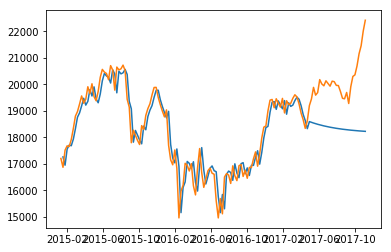
\includegraphics[width=.9\linewidth]{./obipy-resources/cAoUWN.png}
\end{center}

 この図を見るとモデルは与えられたデータに対してかなり適合していることがわかるが、予測の段階で非常に大きな誤差が生まれていることがわかる。 \ref{sec:org0f3006e} p, q の決定法 に書かれている規則を考えるとこのモデルには単位根が残っている可能性が考えられる。これについては次に行う Random Forest を用いた回帰予測とこれらのモデルの精度比較を行った後、 SARIMA モデルと合わせて検討を行う。\\

 同様に比較として Random Forest 回帰を用いた予測を行う。今回は \textcircled{\scriptsize 1} における ARIMA モデル の係数 p の値に従い \footnote{少なくとも過去の値一つと比較した際に何らかの相関があると考えられるためである。} 説明変数に過去の値を一つ取ってモデルを作成した。\\

\begin{minted}[frame=lines,linenos=true,obeytabs,tabsize=4]{python}
ts1_s1 = ts1.shift(1).dropna()[:120]
ts1_y = ts1[1:][:120]
r_forest2 = RandomForestRegressor(n_estimators = 1000, criterion = 'mse',
                                  random_state = 1, n_jobs = 1)
r_forest.fit(np.vstack((ts1_s1.values)),ts1_y.values)
ts1_pred_with_RF2 = r_forest.predict(np.vstack((ts1.shift(1).dropna().values)))
ts1_pred_with_RF2_dataframe = \
    pd.DataFrame({'Close': ts1_pred_with_RF2.T.tolist()},
                 index =  pd.DatetimeIndex(periods = 147,
                                           freq = 'W', start = '2015-1-18'))
plt.hold(True)
plt.plot(ts1_pred_with_RF2_dataframe)
plt.plot(ts1)
\end{minted}

%\begin{verbatim}
%[<matplotlib.lines.Line2D at 0x7fbda609c278>]
%\end{verbatim}
\begin{center}
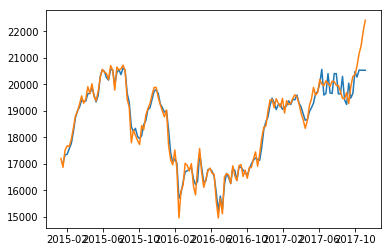
\includegraphics[width=.9\linewidth]{./obipy-resources/YbLLZi.png}
\end{center}

 このグラフを見ると、ARIMAモデルを用いた場合に対してもより精度が良くなっているように見える。予測部分に関してもそれなりに近い動きを示しているが、やや不安定な動きを見せている。\\

 次にモデルとの適合具合を調べるために MSE (二乗平均誤差) \footnote{Mean Squared Error} を取る。\\
\begin{minted}[frame=lines,linenos=true,obeytabs,tabsize=4]{python}
train_with_RF_resid = ts1[1:][:120] - ts1_pred_with_RF[:120]
train_with_ARMA_resid = ts1[1:][:120] - ts1_pred_with_ARMA_dataframe.tolist()[:120]
train_with_RF2_resid = ts1[1:][:120] - ts1_pred_with_RF2[:120]
MSE_train_RF = np.array([(elem * elem) for elem in train_with_RF_resid]).mean()
MSE_train_ARMA = np.array([(elem * elem) for elem in train_with_ARMA_resid]).mean()
MSE_train_RF2 = np.array([(elem * elem) for elem in train_with_RF2_resid]).mean()
print('train: MSE')
print('RandomForest and ARIMA model: ', MSE_train_RF)
print('      AR(I)MA model         : ', MSE_train_ARMA)
print('      Random Forest         : ', MSE_train_RF2)
\end{minted}

train: MSE\\
RandomForest and ARIMA model:  1210139.138746533\\
      AR(I)MA model         :  247038.67430585716\\
      Random Forest         :  42615.21572554316\\

 この結果から、提案した手法が元データを学習する面で良い精度を得られたなかったことは明らかである。また、 ARIMA モデルの精度が低いように見えるが、これは ARIMA モデルが 元データに対してずれた結果を示しているためであると考えられる。実施に求めた時系列データを一つずらすことで以下の結果を得ることが出来る。\\

\begin{minted}[frame=lines,linenos=true,obeytabs,tabsize=4]{python}
ts1_pred_with_ARMA_dataframe2 = ts1_arima.predict('2015-1-18','2017-11-5')
train_with_ARMA_resid2 = ts1[:120] - ts1_pred_with_ARMA_dataframe2.tolist()[:120]
MSE_train_ARMA2 = np.array([(elem * elem) for elem in train_with_ARMA_resid2]).mean()
print('train: MSE')
print('      AR(I)MA model?        : ', MSE_train_ARMA2)
\end{minted}

train: MSE\\
      AR(I)MA model?        :  8580.270341196769\\

 この結果は Random Forest に比べてもかなり良い結果であることがわかる。\\
 次に予測に関する精度を比較する。こちらも同様に MSE を用いた比較を行っている。\\
\begin{minted}[frame=lines,linenos=true,obeytabs,tabsize=4]{python}
pred_with_RF_resid = ts1[1:][120:] - ts1_pred_with_RF[120:]
pred_with_ARMA_resid = ts1[1:][120:] - ts1_pred_with_ARMA_dataframe.tolist()[120:]
pred_with_RF2_resid = ts1[1:][120:] - ts1_pred_with_RF2[120:]
MSE_pred_RF = np.array([(elem * elem) for elem in pred_with_RF_resid]).mean()
MSE_pred_ARMA = np.array([(elem * elem) for elem in pred_with_ARMA_resid]).mean()
MSE_pred_RF2 = np.array([(elem * elem) for elem in pred_with_RF2_resid]).mean()
print('predict: MSE')
print('RandomForest and ARIMA model: ', MSE_pred_RF)
print('      AR(I)MA model         : ', MSE_pred_ARMA)
print('      Random Forest         : ', MSE_pred_RF2)

pred_with_ARMA_resid2 = ts1[1:][120:] - ts1_pred_with_ARMA_dataframe2.tolist()[120:]
MSE_pred_ARMA2 = np.array([(elem * elem) for elem in pred_with_ARMA_resid2]).mean()
print('      AR(I)MA model?        : ', MSE_pred_ARMA2)
\end{minted}

predict: MSE\\
RandomForest and ARIMA model:  7288573.59721489\\
      AR(I)MA model         :  4002781.362739798\\
      Random Forest         :  415257.4516347963\\
      AR(I)MA model?        :  4002781.362739798\\

 この結果からはそれぞれの図で確認したとおり、 Random Forest が最も良い精度を持っていることがわかる。また ARIMA モデルは、モデルの元データとの適合度においては求まったデータをずらすことで精度が大幅に向上したが、予測の観点ではずらしても良い精度を得られていないことがわかる。\\

 今回の実験における ARIMA モデルの精度について確認が出来たところで SARIMA モデルを用いた検討を行う。まず SARIMA モデルを適用するべきであるのかを確認するために ACF, PACF のグラフを確認する。\\

\begin{minted}[frame=lines,linenos=true,obeytabs,tabsize=4]{python}
from statsmodels.graphics.tsaplots import plot_acf, plot_pacf
fig = plt.figure(figsize = (12,8))
ax1 = fig.add_subplot(211)
fig = sm.graphics.tsa.plot_acf(ts1, lags=40, ax = ax1)
ax2 = fig.add_subplot(212)
fig = sm.graphics.tsa.plot_pacf(ts1, lags=40, ax = ax2)
\end{minted}

\begin{center}
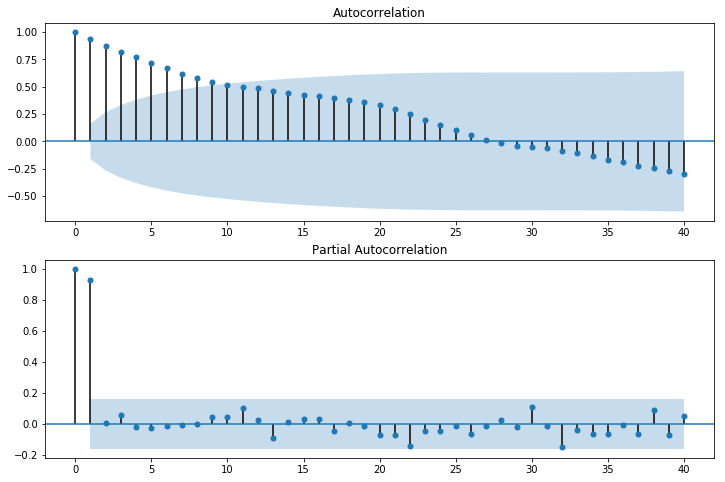
\includegraphics[width=.9\linewidth]{./obipy-resources/xBGhjB.png}
\end{center}

 この結果を注視すると、PACF のグラフに微かに周期性を見ることが出来る。よって 季節階差\footnote{正確にはこのデータは週次ごとのデータなので、``季節''差分を取っているわけではなく、周期性に基づいて階差を取っている。} を取ることが出来ると考えられる。\\
 実際に SARIMA モデルを適用すると以下のようになる。尚 実験の結果 \footnote{様々なモデルを作成し、最もAICの小さいモデルを選択した} 、このデータに対して季節成分の係数 (P,D,Q) は (1, 1, 0) を設定している。\\
\begin{minted}[frame=lines,linenos=true,obeytabs,tabsize=4]{python}
ts1_SARIMA = sm.tsa.SARIMAX(ts1, order=(1,0,0), seasonal_order=(1,1,0,12)).fit()
ts1_pred_with_SARIMA_dataframe =  ts1_SARIMA.predict('2015-1-18','2017-11-5')

plt.hold(True)
plt.plot(ts1_pred_with_SARIMA_dataframe)
plt.plot(ts1)
\end{minted}

%\begin{verbatim}
%[<matplotlib.lines.Line2D at 0x7fbda3f561d0>]
%\end{verbatim}
\begin{center}
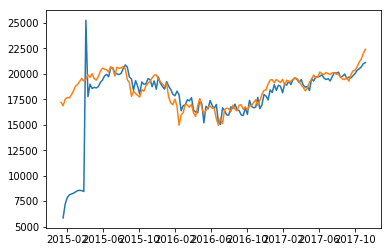
\includegraphics[width=.9\linewidth]{./obipy-resources/FRNY3r.png}
\end{center}

 結果より時系列的に始めに近い部分の値が不安定ではあるが、それ以外の値に関しては元データに即した値を求めると考えられ、予測も比較的理想に近い値を取っている。\\
 また、不安定な部分を除いて表示を行うと以下のようになる。\\
\begin{minted}[frame=lines,linenos=true,obeytabs,tabsize=4]{python}
plt.plot(ts1_pred_with_SARIMA_dataframe[15:])
plt.plot(ts1[15:])
\end{minted}

%\begin{verbatim}
%[<matplotlib.lines.Line2D at 0x7fbda3ebd710>]
%\end{verbatim}
\begin{center}
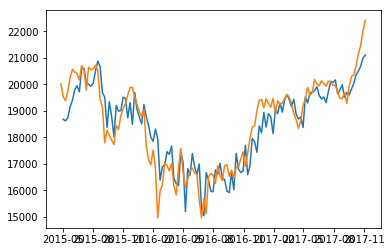
\includegraphics[width=.9\linewidth]{./obipy-resources/fFVOJA.png}
\end{center}

 次にこの不安定な部分を取り除いた場合の SARIMA モデルについて MSE を求める。\\
始めに近い値を取り除くことが出来ると考えた理由は、季節差分を取った際に初期のデータは比較される側のみであり、それ以降のデータとは扱いが異なるためである。\\

\begin{minted}[frame=lines,linenos=true,obeytabs,tabsize=4]{python}
pred_with_SARIMA_resid2 = ts1[15:][1:][105:] - ts1_pred_with_SARIMA_dataframe.tolist()[15:][105:]
MSE_pred_SARIMA = np.array([(elem * elem) for elem in pred_with_SARIMA_resid2]).mean()
print('train: MSE')
print('      SARIMA model?        : ', MSE_pred_SARIMA)
pred_with_SARIMA_resid2 = ts1[15:][1:][:105] - ts1_pred_with_SARIMA_dataframe.tolist()[15:][:105]
MSE_pred_SARIMA = np.array([(elem * elem) for elem in pred_with_SARIMA_resid2]).mean()
print('predict: MSE')
print('      SARIMA model?        : ', MSE_pred_SARIMA)
\end{minted}

train: MSE\\
      SARIMA model?        :  256194.51962546672\\
predict: MSE\\
      SARIMA model?        :  571242.1110044359\\

 この結果から、少なくとも ARIMA モデルに比べると SARIMA モデルが精度面で高い性能を示していると考えることが出来る。\\
\printbibliography
Emacs 26.0.91 (Org mode 9.1.6)
\end{document}
